
\begin{tcolorbox}[colback=primaryColor,colframe=primaryColor,arc=3mm,halign=center,valign=center,height=2.5cm]
    \color{white}\LARGE\bfseries CONFRONTO BEFORE/AFTER \\[0.2cm]
    \color{white!80}\large UX Design Project: Help People Help People --- TPER S.p.A. \\[0.1cm]
    \color{white!60}\normalsize Phase C --- Design Proposal
\end{tcolorbox}

\vspace{0.5cm}

\section{Introduzione}

Questo confronto Before/After mette in evidenza le differenze tra il sito \texttt{tper.it} attuale e la proposta di redesign \texttt{tper 2.0}, sviluppata a partire dalle 13 raccomandazioni R1--R13 (Phase B). Ogni sezione è ancorata alle evidenze Phase A: 4 soggetti testati, solo \textbf{6/20 task completati (30\%)}, \textbf{SUS medio 37.5/100} --- ben al di sotto della soglia di accettabilità. Gli use case UR-01--UR-05 hanno guidato le scelte progettuali.

\vspace{0.2cm}

\textbf{Ecosistema TPER:} \texttt{tper.it} è un sito \textit{puramente informativo} --- non consente acquisti diretti. Le transazioni avvengono su 5 canali specializzati:
\begin{itemize}[nosep]
    \item \texttt{solweb.tper.it} --- abbonamenti online;
    \item \textbf{App Roger} --- biglietti digitali;
    \item \textbf{Punti Tper} --- sportelli fisici;
    \item \textbf{Tabaccherie / PuntoLis} --- ricariche;
    \item \textbf{Contactless a bordo} --- pagamento immediato.
\end{itemize}
Il redesign trasforma \texttt{tper.it} da contenitore generico di notizie a \textbf{hub informativo e guida attiva all'ecosistema}.

\vspace{0.3cm}

% ============================================================
% CONFRONTO 1: HOMEPAGE tper.it
% ============================================================
\section{Home Page \texttt{tper.it}}
\label{sec:comparison-home}

\textbf{D1 $\rightarrow$ R1} --- Home caotica (P5,I5) $\rightarrow$ Home task-oriented. Maria: \textit{``non so da dove cominciare''}, SUS medio 37.5/100.

\begin{figure}[H]
\centering
\begin{minipage}[t]{0.498\textwidth}
\centering
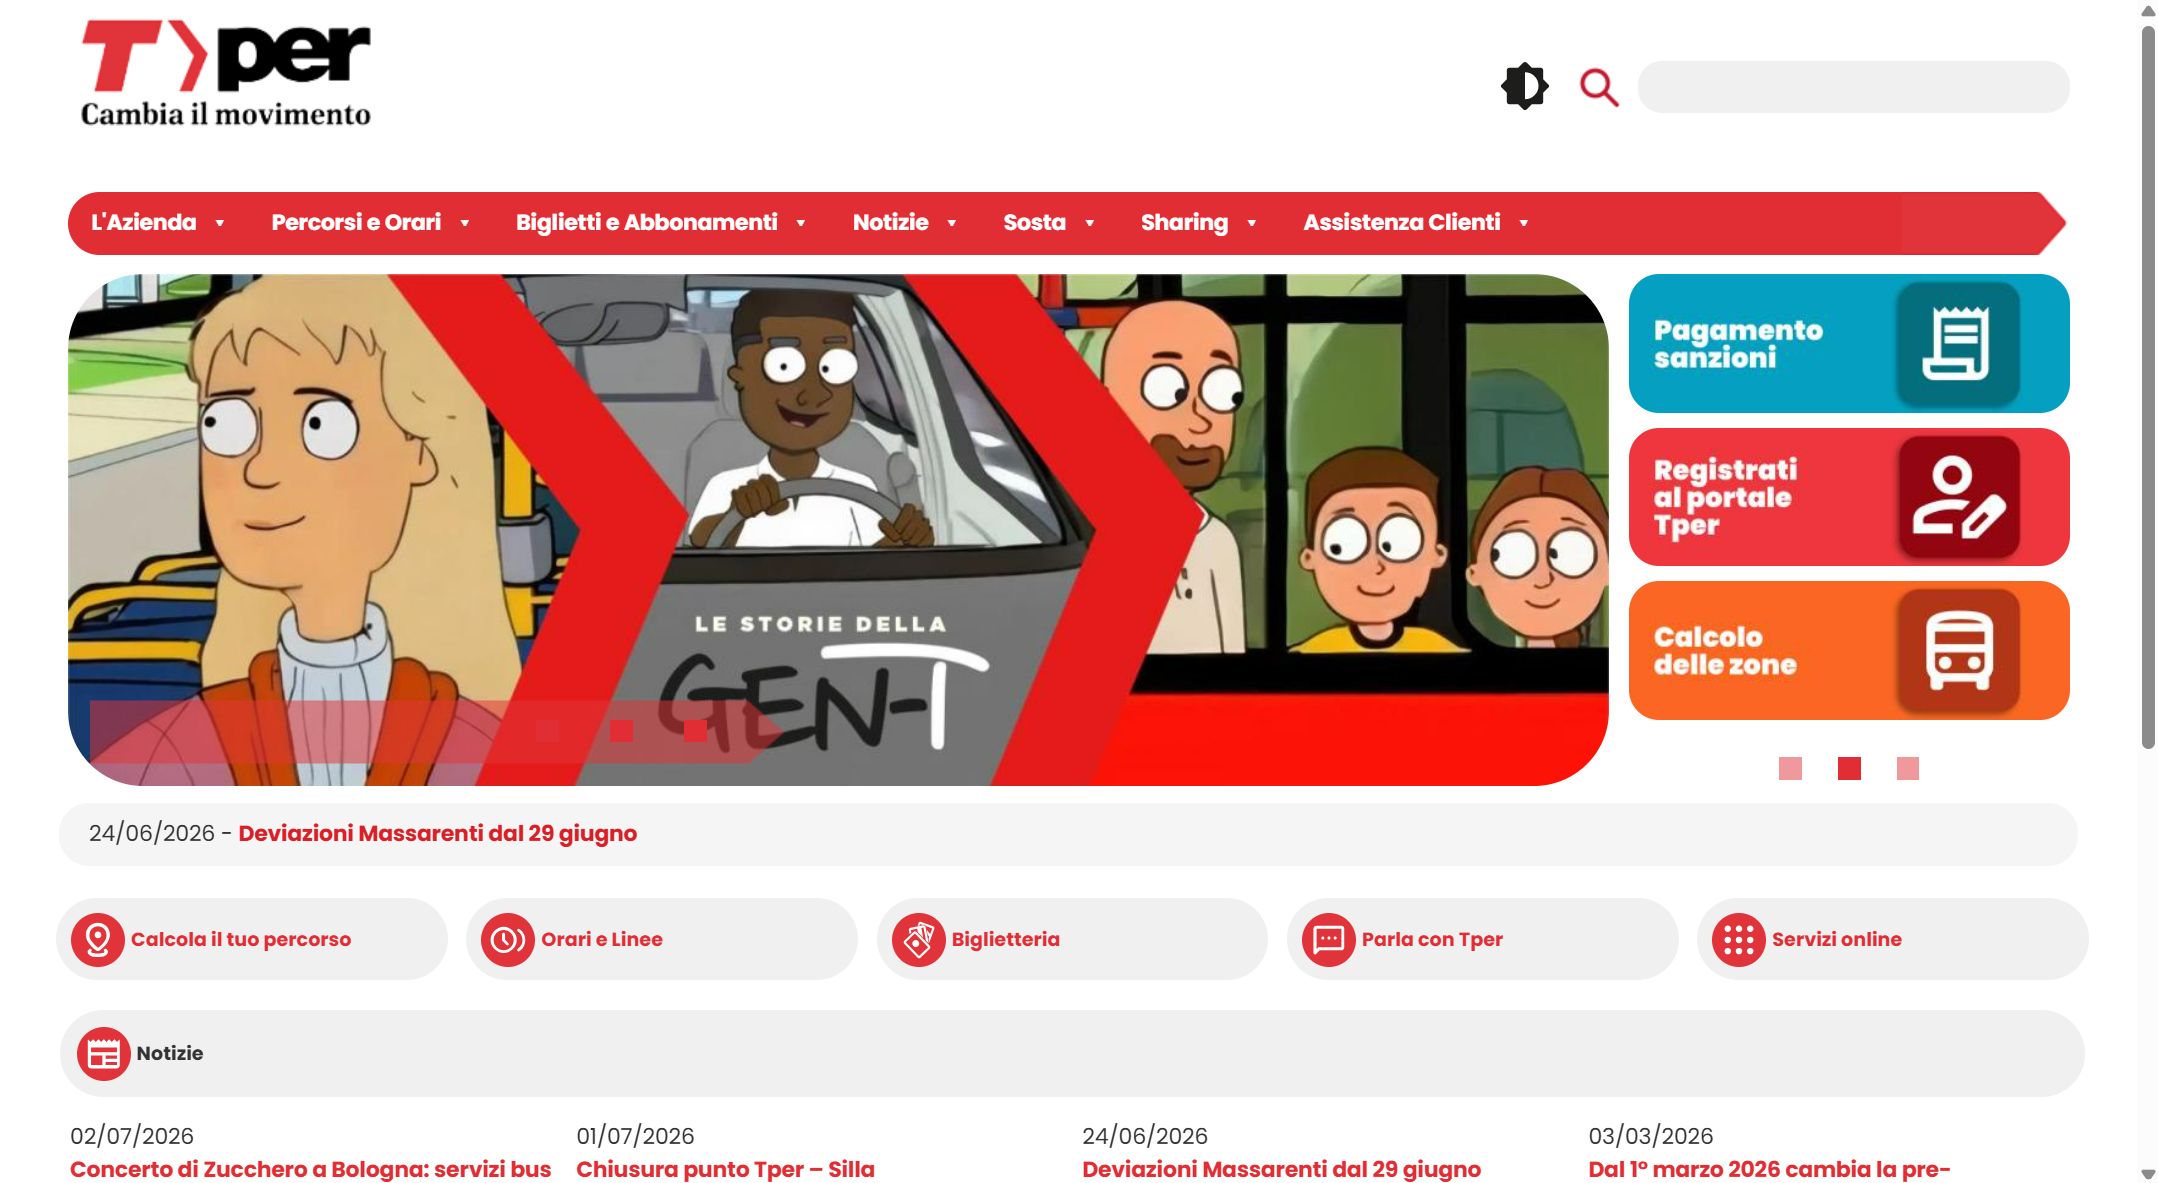
\includegraphics[width=\textwidth]{Tper sito originale/Homepage.png}
\par\small\textit{Before: \texttt{tper.it} live --- slider di news aziendali, nessuna CTA primaria}
\end{minipage}
\hfill
\begin{minipage}[t]{0.498\textwidth}
\centering
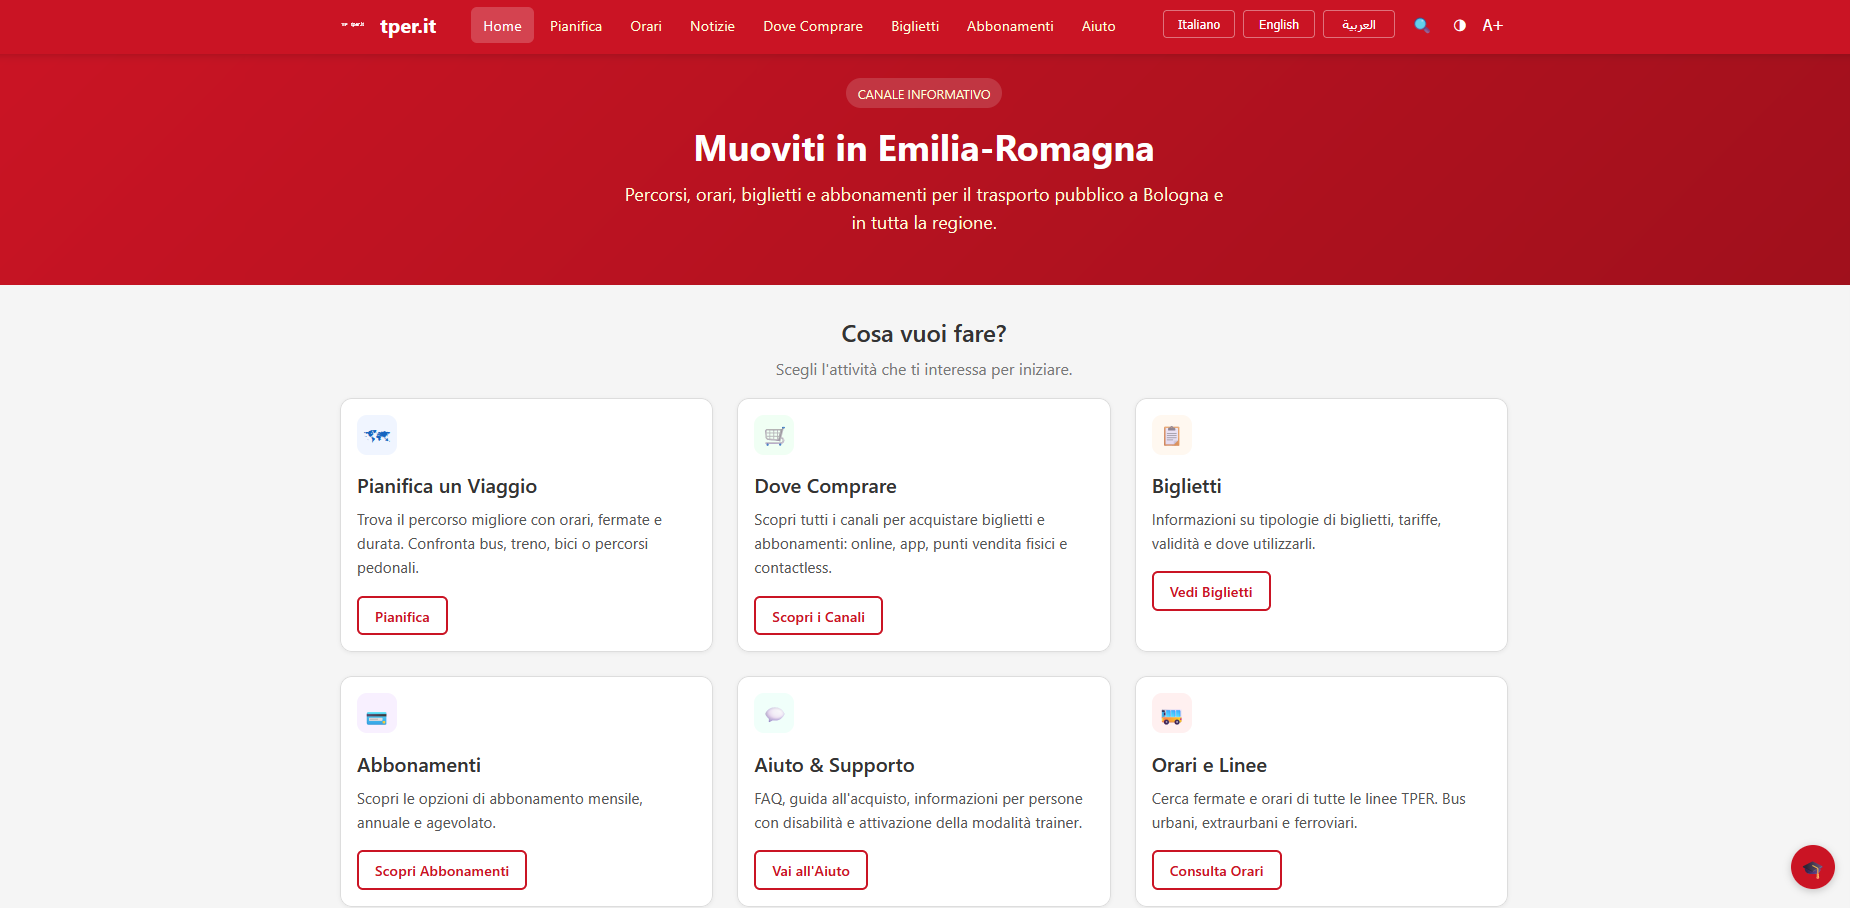
\includegraphics[width=\textwidth]{Redesign Tper 2.0/homepage.png}
\par\small\textit{After: tper 2.0 --- hero pianificatore + griglia 6 card task-oriented}
\end{minipage}
\caption{Homepage \texttt{tper.it}}
\label{fig:comparison-home}
\end{figure}

\begin{table}[H]
\centering
\small
\renewcommand{\arraystretch}{1.4}
\begin{tabular}{|p{0.5cm}|p{7cm}|p{7cm}|}
\hline
& \textbf{Before} & \textbf{After} \\ \hline
\cellcolor{primaryColor!15} &
\textit{Homepage attuale di \texttt{tper.it} (live)} &
\textit{Homepage redesign \texttt{tper 2.0}} \\ \hline

\raisebox{0.5cm}{\rotatebox{90}{\textbf{Contenuti}}} &
Slider di notizie aziendali, comunicati stampa, bandi di gara occupano la homepage. Il pianificatore di viaggio è raggiungibile dopo 2--3 click attraverso \textit{Percorsi e Orari} $\rightarrow$ \textit{Calcola il tuo percorso}. Nessuna gerarchia tra contenuti utente e contenuti istituzionali (Issue D1). &
Hero section dedicata al pianificatore di viaggio con campi ``Partenza'' e ``Destinazione'' già visibili. Griglia ``Cosa vuoi fare?'' con 6 card task-oriented: Pianifica, Dove Comprare, Biglietti, Abbonamenti, Aiuto, Orari. News aziendali spostate in sezione separata (R1). \\ \hline

\raisebox{0.5cm}{\rotatebox{90}{\textbf{CTA}}} &
Link testuali generici: ``Servizi online'', ``Percorsi e Orari'', ``Biglietteria'', ``Parla con Tper''. L'utente deve interpretare la terminologia aziendale per capire dove andare (Issue D3). &
Pulsanti grandi con icone e linguaggio utente: ``Pianifica un Viaggio'', ``Dove Comprare?'', ``Vedi Biglietti'', ``Scopri Abbonamenti'', ``Vai all'Aiuto'', ``Consulta Orari''. Ogni card mostra un'icona distintiva colorata (R2, R9). \\ \hline

\raisebox{0.5cm}{\rotatebox{90}{\textbf{Navigazione}}} &
Mega-menu con 7 voci principali e oltre 50 sottovoci, dominato da contenuti istituzionali: \textit{Società Trasparente}, \textit{Appalti e Fornitori}, \textit{L'Azienda} occupano la maggior parte dello spazio. L'utente si perde tra contenuti legali (Issue D2). &
Navigazione flat a 8 voci task-oriented: Home, Pianifica, Orari, Notizie, \textbf{Dove Comprare}, Biglietti, Abbonamenti, Aiuto. Breadcrumb su tutte le pagine interne per orientamento. Contenuti istituzionali disponibili via footer (R2, R3). \\ \hline

\raisebox{0.5cm}{\rotatebox{90}{\textbf{Info}}} &
Nessuna indicazione sul ruolo informativo del sito. L'utente cerca funzioni transazionali che non esistono su \texttt{tper.it} (UR-01, UR-03). &
Banner esplicito su ogni pagina: ``\texttt{tper.it} è un sito informativo. Per acquistare biglietti e abbonamenti utilizza uno dei canali dedicati'' con link a Dove Comprare. Hero badge: ``CANALE INFORMATIVO'' (R1). \\ \hline
\end{tabular}
\caption{Homepage (\texttt{tper.it} live vs tper 2.0)}
\label{tab:comparison-home}
\end{table}

\vspace{0.3cm}

% ============================================================
% CONFRONTO 2: HOMEPAGE solweb
% ============================================================
\section{Home Page \texttt{solweb.tper.it}}
\label{sec:comparison-solweb-home}

\textbf{D5 $\rightarrow$ R7} --- Login obbligatorio (P3,I5) $\rightarrow$ Guest path + 4 azioni rapide. 3/4 falliti T3, transizione \texttt{tper.it}$\rightarrow$\texttt{solweb} non segnalata.

\begin{figure}[H]
\centering
\begin{minipage}[t]{0.498\textwidth}
\centering
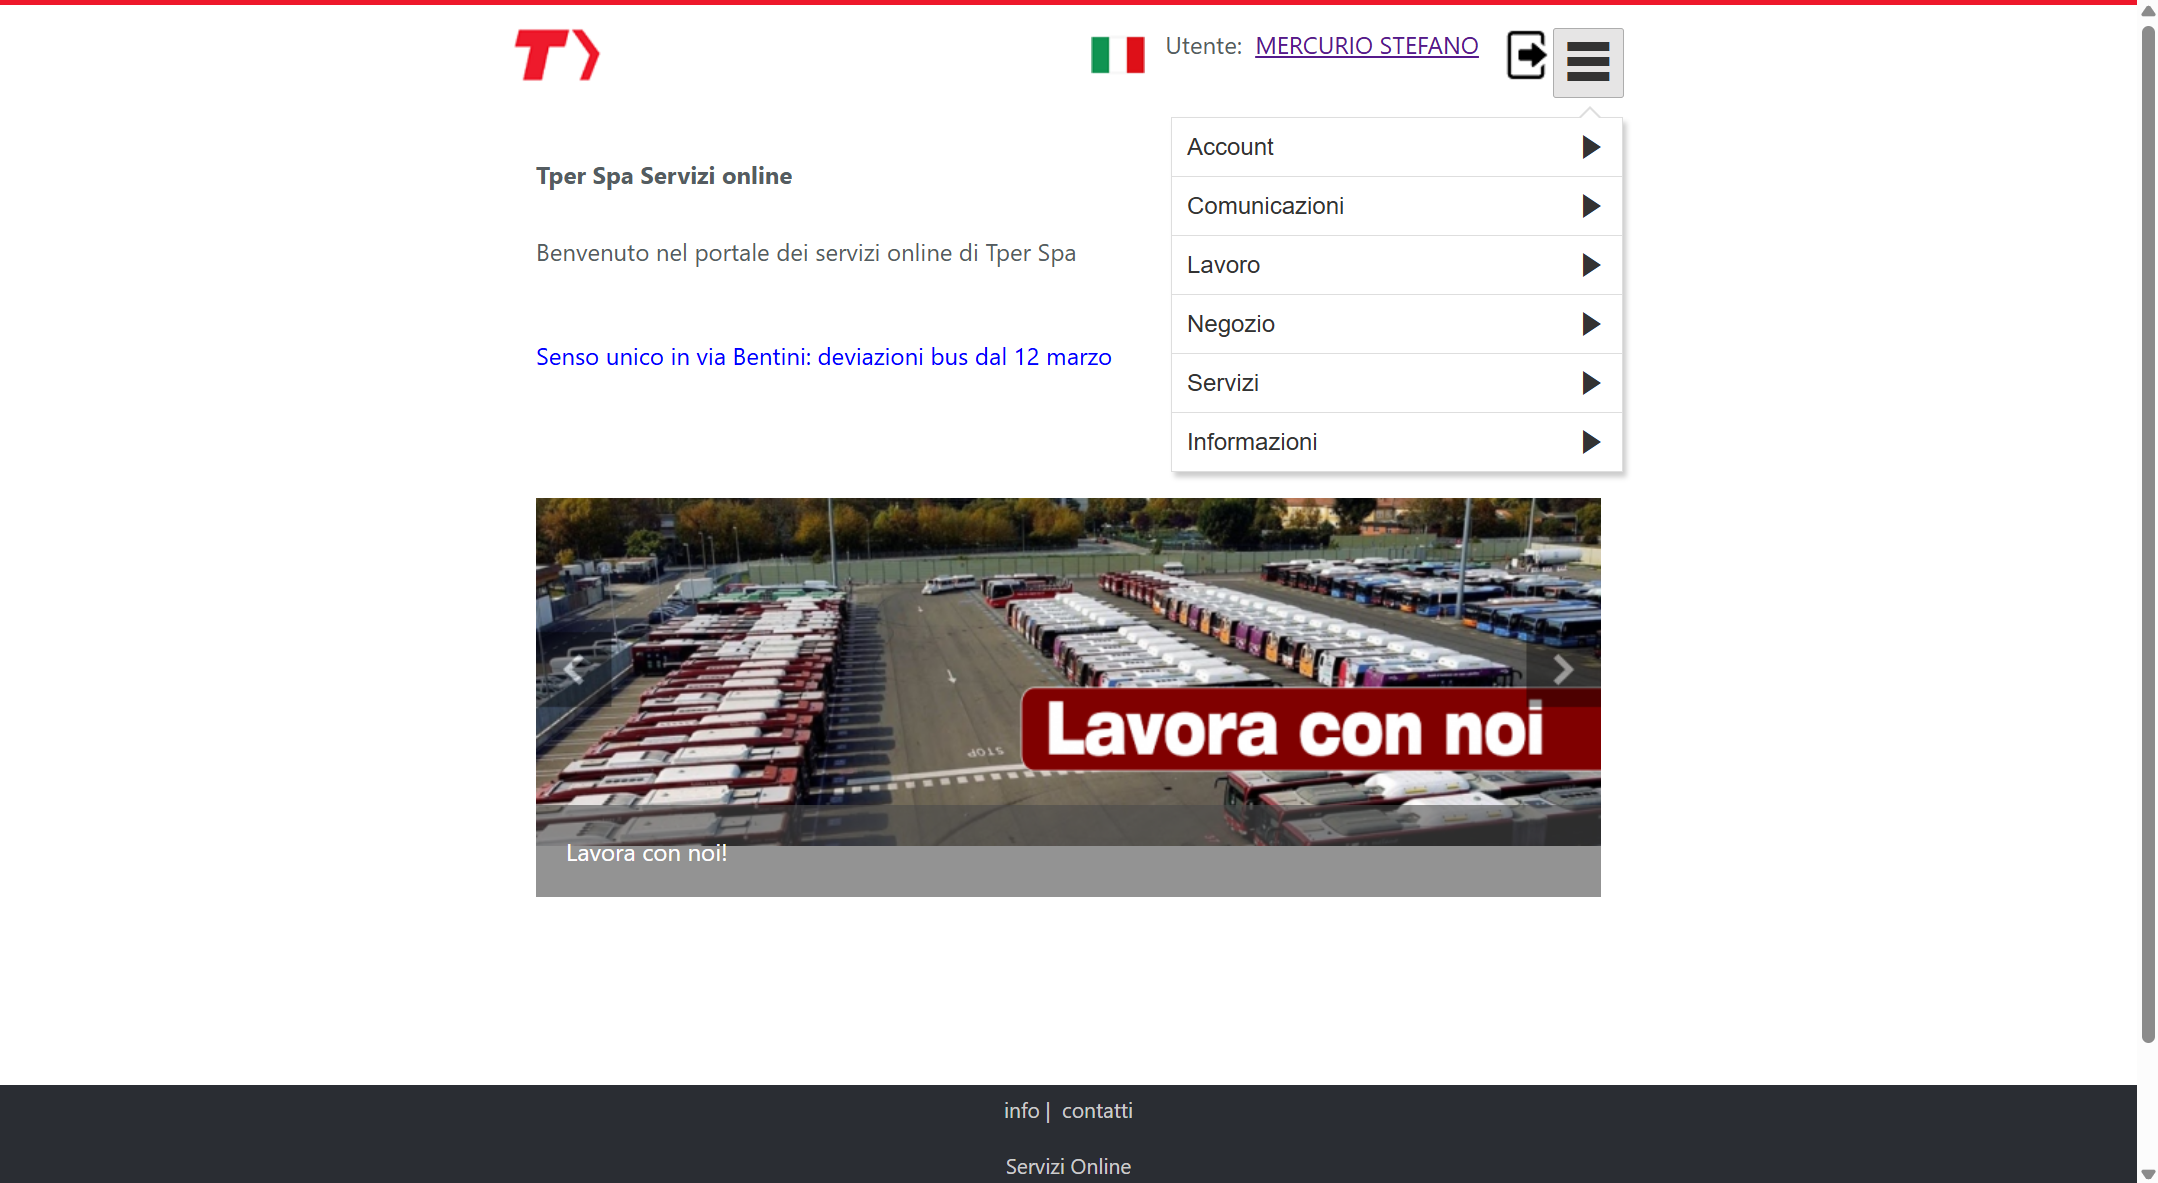
\includegraphics[width=\textwidth]{Tper sito originale/HomepageS.png}\\[2pt]
{\small\textit{+ seconda vista:}}\\[2pt]
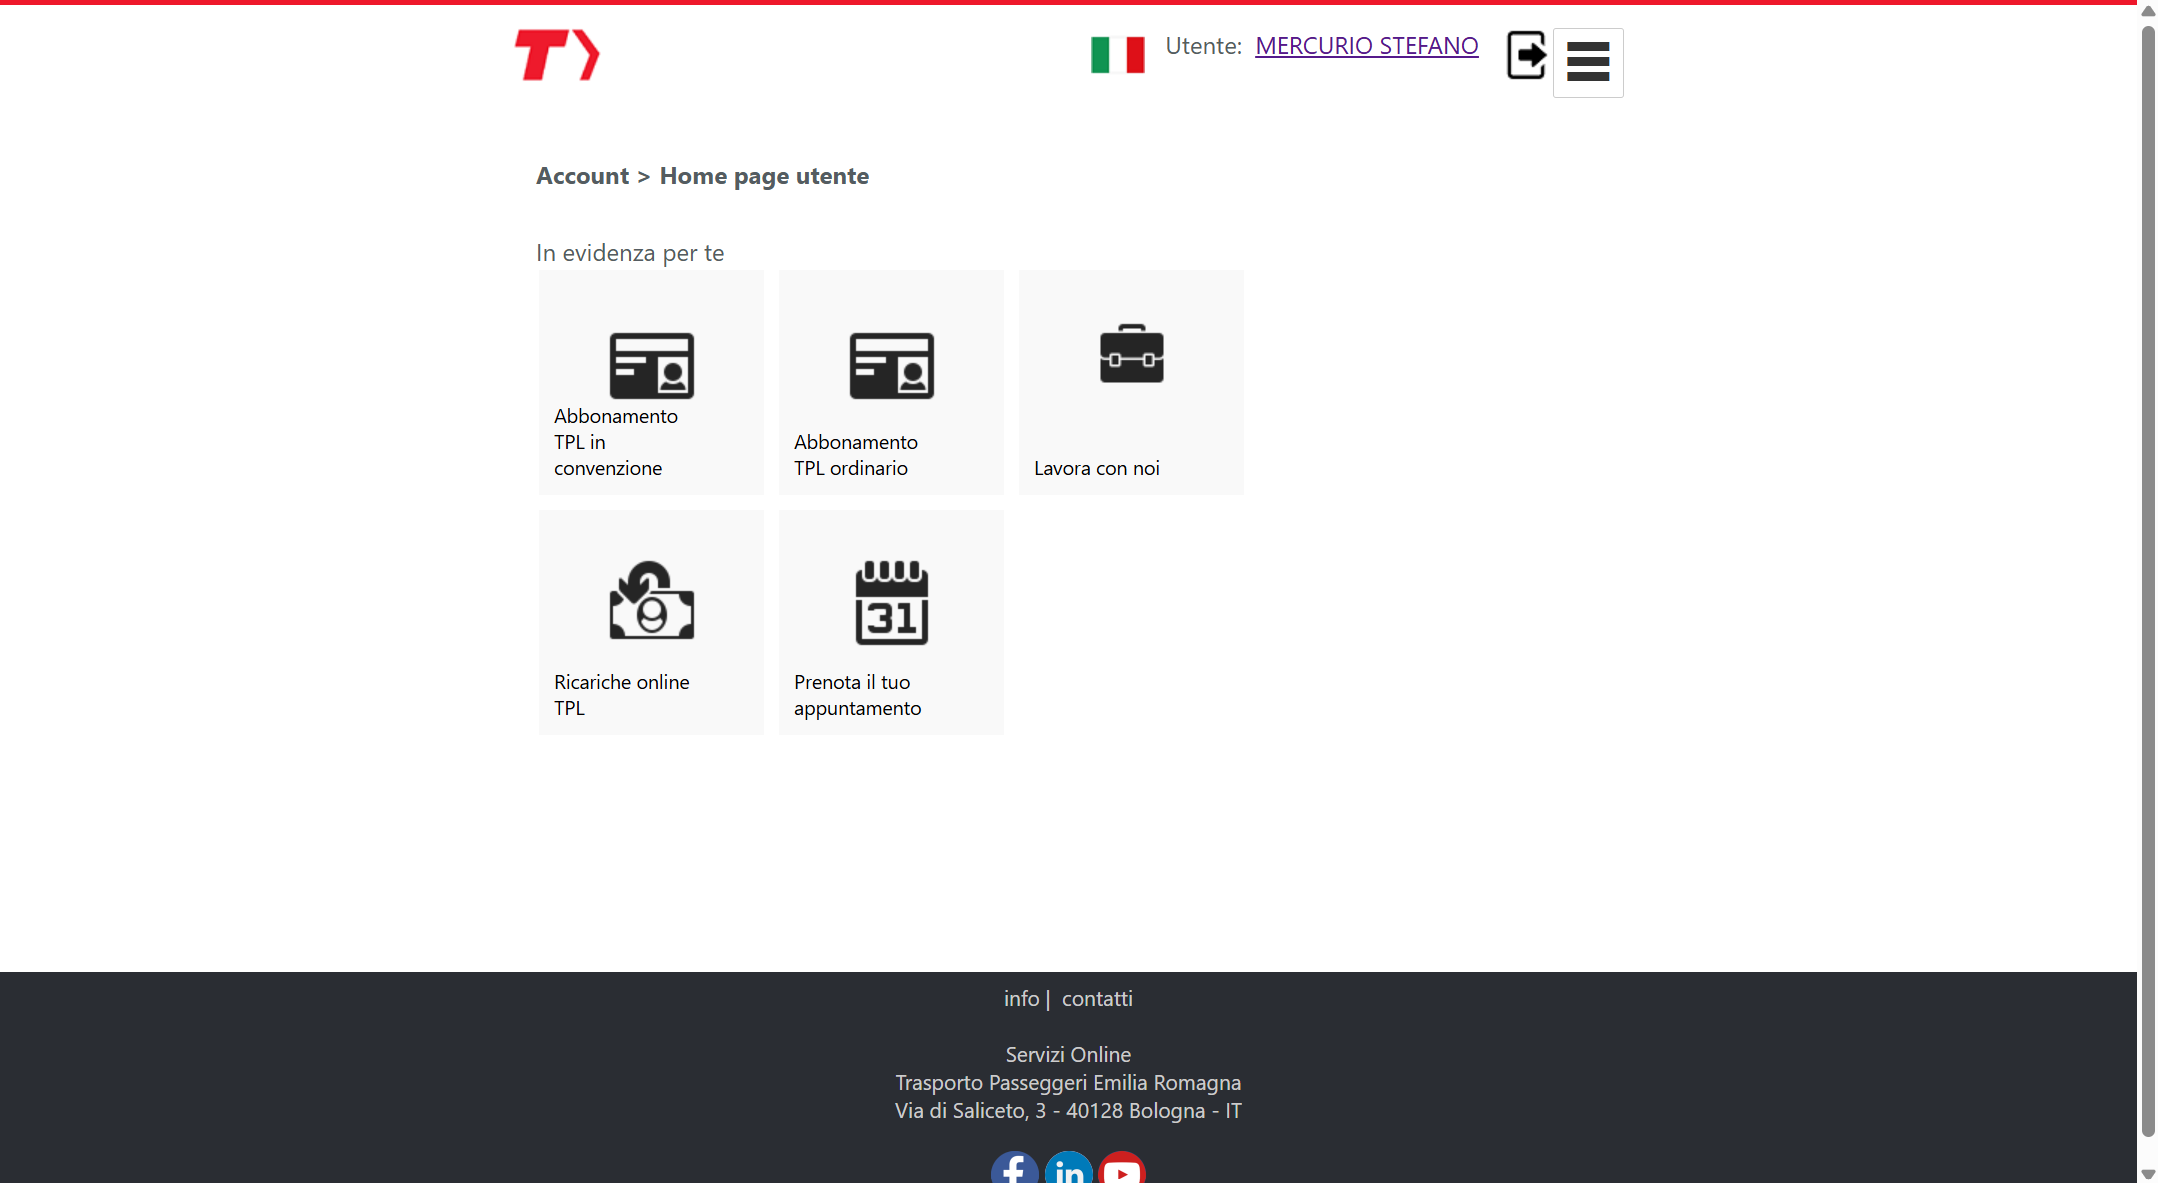
\includegraphics[width=\textwidth]{Tper sito originale/HomepageS2.png}
\par\small\textit{Before: \texttt{solweb} originale --- login obbligatorio, nessun percorso guest}
\end{minipage}
\hfill
\begin{minipage}[t]{0.498\textwidth}
\centering
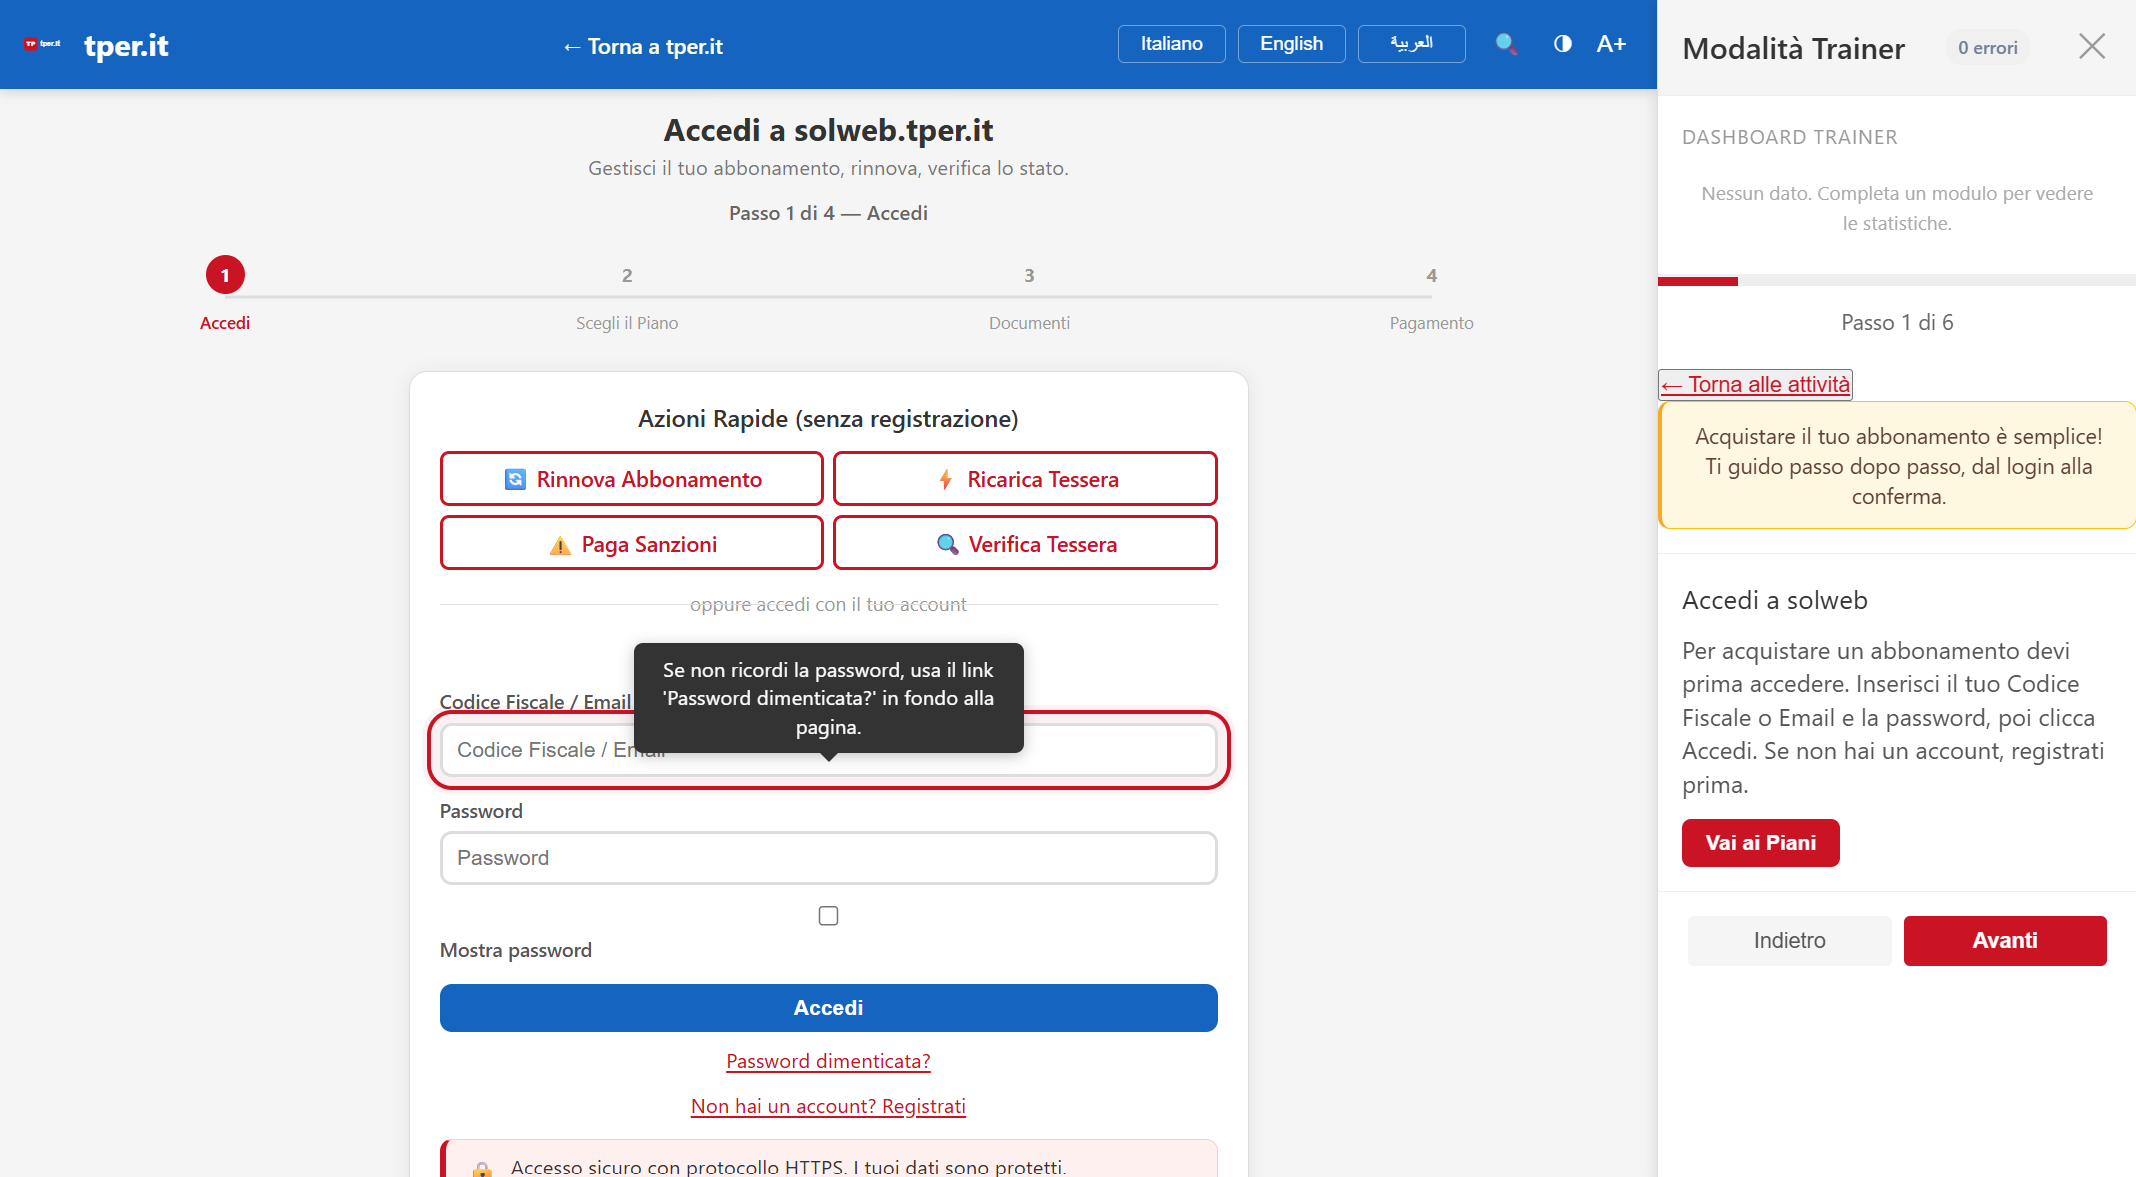
\includegraphics[width=\textwidth]{Redesign Tper 2.0/HomepageS.png}
\par\small\textit{After: solweb 2.0 --- login + 4 azioni rapide senza registrazione}
\end{minipage}
\caption{Homepage \texttt{solweb.tper.it}}
\label{fig:comparison-solweb-home}
\end{figure}

\begin{table}[H]
\centering
\small
\renewcommand{\arraystretch}{1.4}
\begin{tabular}{|p{0.5cm}|p{7cm}|p{7cm}|}
\hline
& \textbf{Before} & \textbf{After} \\ \hline
\cellcolor{primaryColor!15} &
\textit{Portale solweb originale} &
\textit{solweb 2.0 nel redesign} \\ \hline

\raisebox{0.5cm}{\rotatebox{90}{\textbf{Accesso}}} &
\textbf{Solo login}: username/SPID/CIE obbligatori per qualsiasi operazione. Nessuna alternativa guest. Per un utente anziano a bassa competenza digitale, la richiesta di ``creare un account'' causa abbandono immediato (Issue D5). &
\textbf{4 azioni rapide senza login}: Rinnovo Impersonale, Ricarica Tessera, Paga Sanzioni, Verifica Tessera. Il login resta disponibile per le operazioni che richiedono autenticazione (ISEE, abbonamenti personali). Barra di progresso a 4 passi: Accedi $\rightarrow$ Scegli il Piano $\rightarrow$ Documenti $\rightarrow$ Pagamento (R7). \\ \hline

\raisebox{0.5cm}{\rotatebox{90}{\textbf{Transizione}}} &
Passaggio da \texttt{tper.it} a \texttt{solweb} senza alcun avviso: cambio di dominio, interfaccia, colori e layout. L'utente non capisce se è ancora su TPER (Issue R4). &
\textbf{Modale di transizione} prima di ogni link esterno: ``Stai per uscire da \texttt{tper.it} --- Verrai reindirizzato al canale di acquisto esterno'' con URL di destinazione visibile (R9). Header solweb con link ``$\leftarrow$ Torna a tper.it'' sempre visibile. \\ \hline

\raisebox{0.5cm}{\rotatebox{90}{\textbf{Orientamento}}} &
Nessuna indicazione di dove ci si trova nell'ecosistema. Interfaccia completamente diversa da \texttt{tper.it}, zero segnaletica di continuità. &
Header blu (\#1565C0) distinto dal rosso TPER per segnalare il cambio di piattaforma. Hero badge ``PIATTAFORMA ABBONAMENTI'' nella dashboard. Breadcrumb contestuali. \\ \hline

\raisebox{0.5cm}{\rotatebox{90}{\textbf{Operazioni}}} &
Tutte le operazioni richiedono registrazione. Nessuna distinzione tra operazioni semplici (ricarica, sanzioni) e complesse (ISEE, rinnovo personale). &
\textbf{Separazione guest/authenticated}: ricarica, sanzioni e verifica tessera accessibili senza login. Acquisto e rinnovo personale protetti da autenticazione con spiegazione del perché (R7). \\ \hline
\end{tabular}
\caption{Homepage \texttt{solweb.tper.it}}
\label{tab:comparison-solweb-home}
\end{table}

\vspace{0.3cm}

% ============================================================
% CONFRONTO 3: RISTRUTTURAZIONE IA (3v3)
% ============================================================
\section{Ristrutturazione dell'Architettura Informativa}
\label{sec:comparison-ia-3v3}

\textbf{D2+D3 $\rightarrow$ R2+R9} --- Menu 200+ voci, 5 livelli $\rightarrow$ Nav piatta 8 voci. ``Rete di vendita'' sepolta al 3° livello.

\subsection*{Il Problema Originale}

Nel sito originale, tre pagine si sovrapponevano generando confusione e duplicazione:

\begin{itemize}[nosep]
    \item \textbf{Biglietti}: elencava biglietti + canali di vendita + tariffe --- troppe informazioni per una pagina sola;
    \item \textbf{Abbonamenti}: elencava abbonamenti + canali + tariffe --- stessa duplicazione della pagina Biglietti;
    \item \textbf{Tariffe}: pagina separata con i prezzi, \textbf{ridondante} e scollegata dal contesto d'uso.
\end{itemize}

Risultato: l'utente doveva \textbf{saltare tra 3 pagine} per rispondere a domande come \textit{``quale abbonamento comprare?''} e \textit{``dove lo compro?''}. La guida ai canali (``Rete di vendita'') era sepolta al terzo livello di navigazione.

\subsection*{La Soluzione: Separazione delle Responsabilità}

Il redesign applica il principio \textbf{ogni pagina, un compito} (R2), eliminando ogni duplicazione:

\begin{itemize}[nosep]
    \item \textbf{Biglietti}: \textit{solo} tipologie di biglietto + wizard a 5 domande + filtri per zona/validità/canale;
    \item \textbf{Abbonamenti}: \textit{solo} piani di abbonamento + wizard a 7 domande + verifica agevolazioni;
    \item \textbf{Dove Comprare}: \textbf{nuova sezione dedicata} che raccoglie tutta la guida ai canali --- wizard a 3 domande, 6 card canale, tabella comparativa 5$\times$7.
\end{itemize}

Le \textbf{tariffe} sono state \textbf{integrate} direttamente in Biglietti e Abbonamenti: il prezzo appare nel momento esatto della decisione sul prodotto, non su una pagina separata.

\begin{figure}[H]
\centering
\textbf{Before --- Sito Originale}\\[4pt]
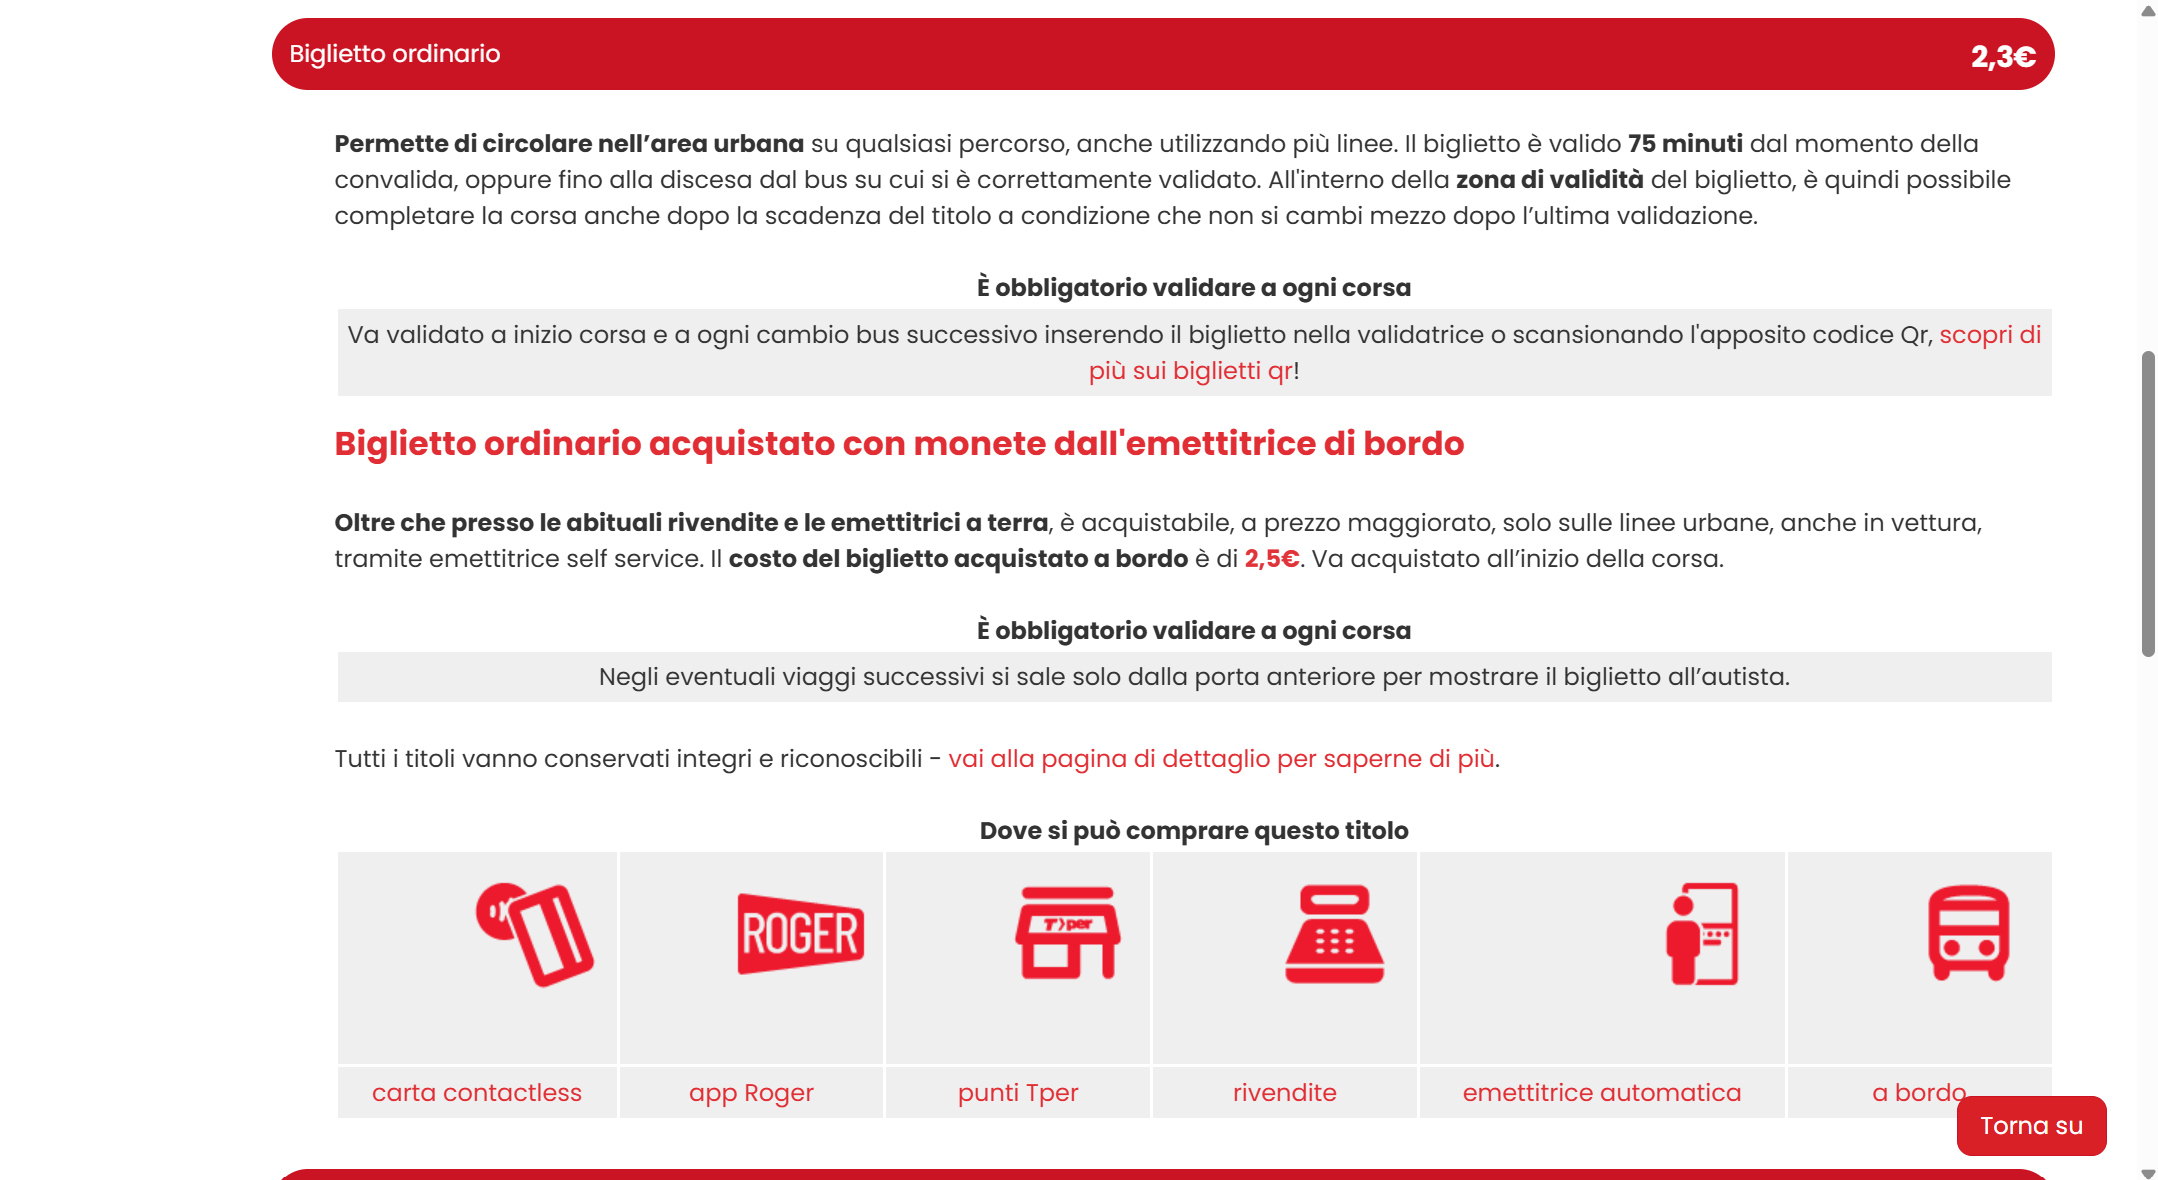
\includegraphics[width=0.332\textwidth]{Tper sito originale/Biglietti.png}\hfill
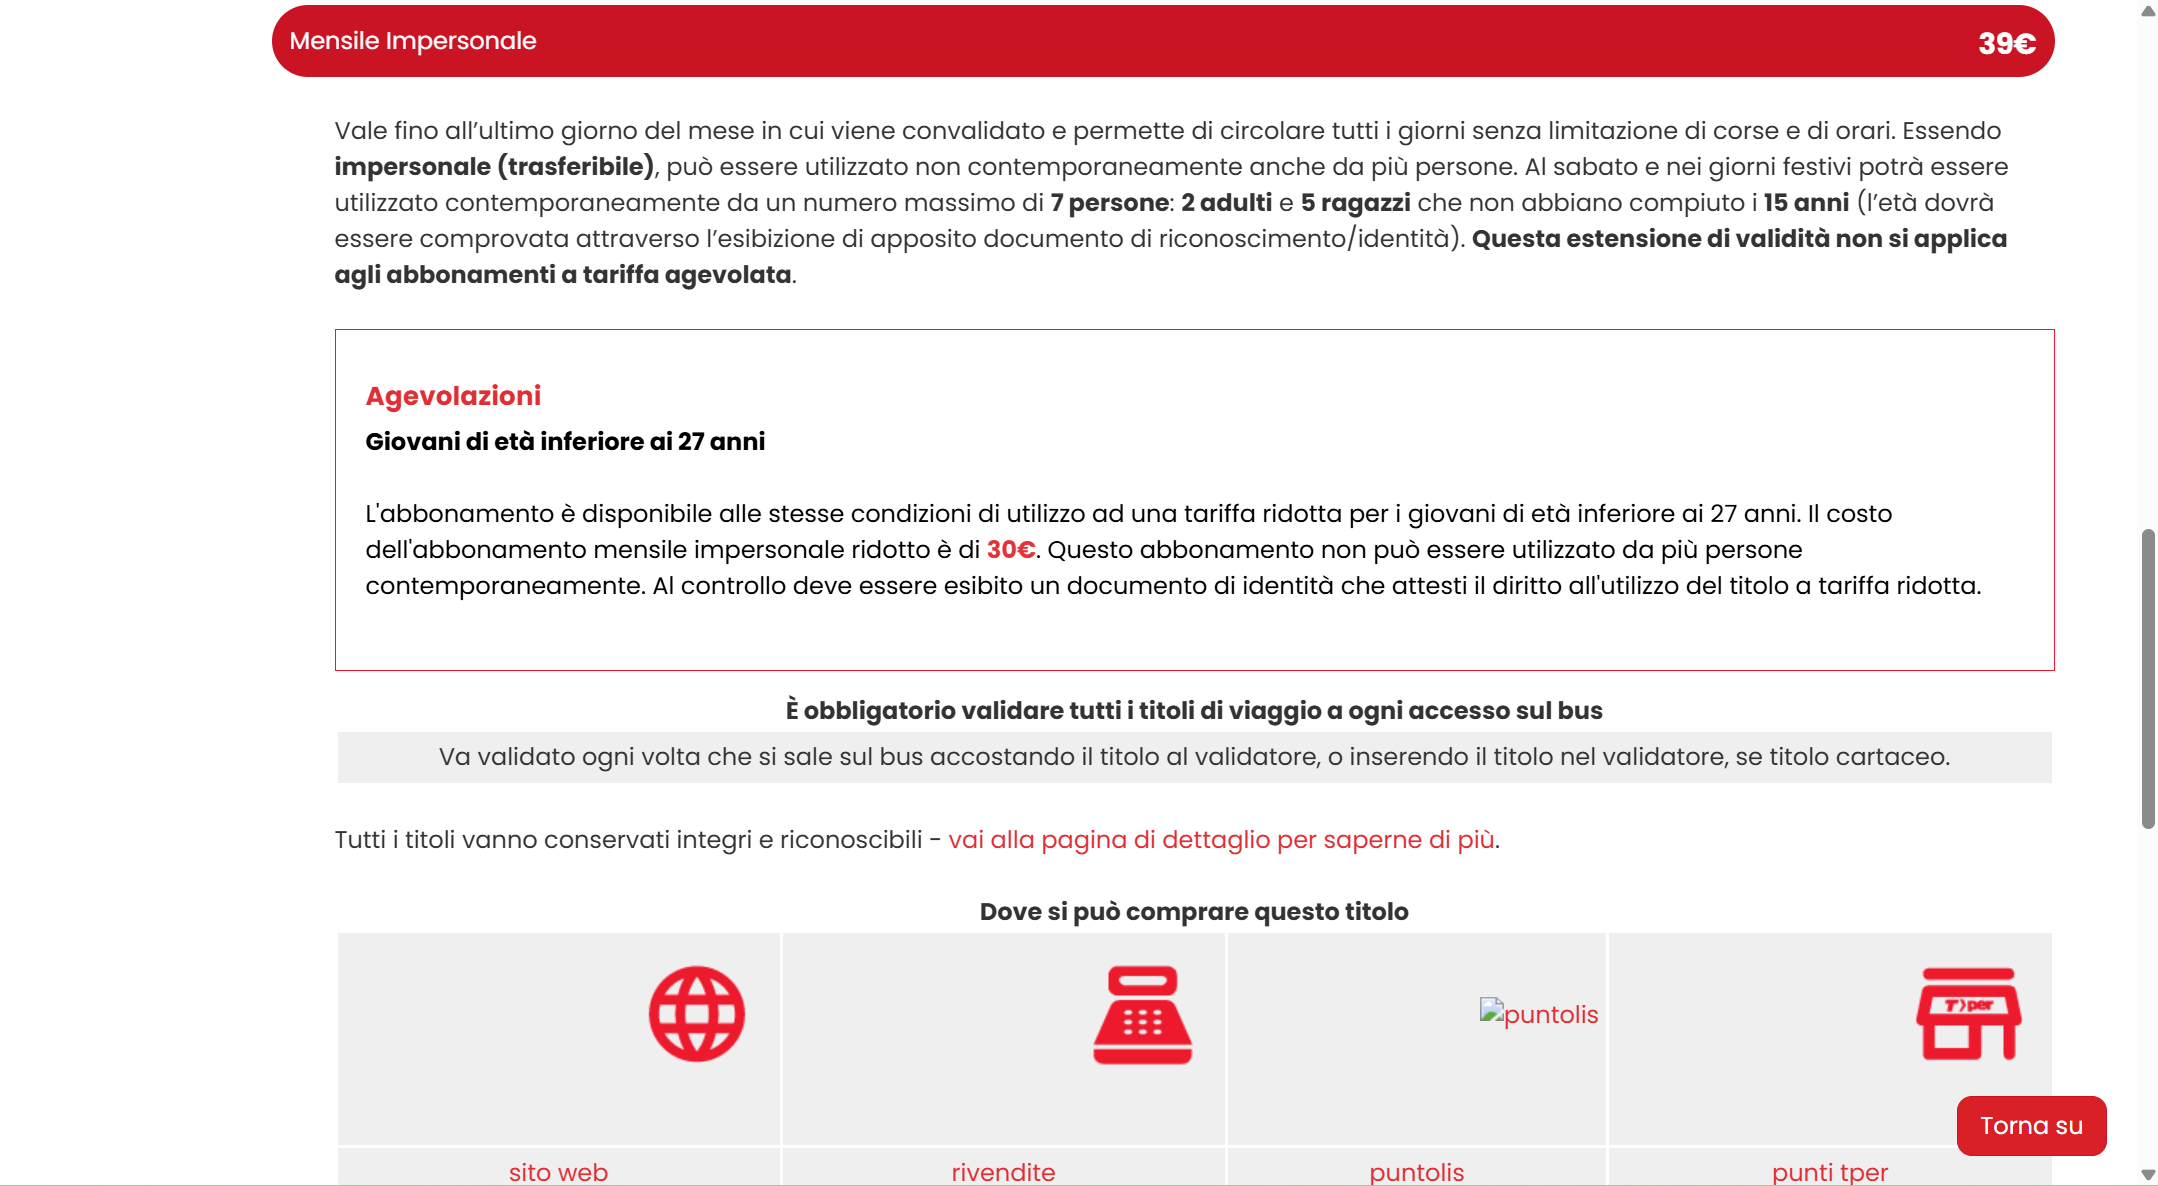
\includegraphics[width=0.332\textwidth]{Tper sito originale/Abbonamenti.png}\hfill
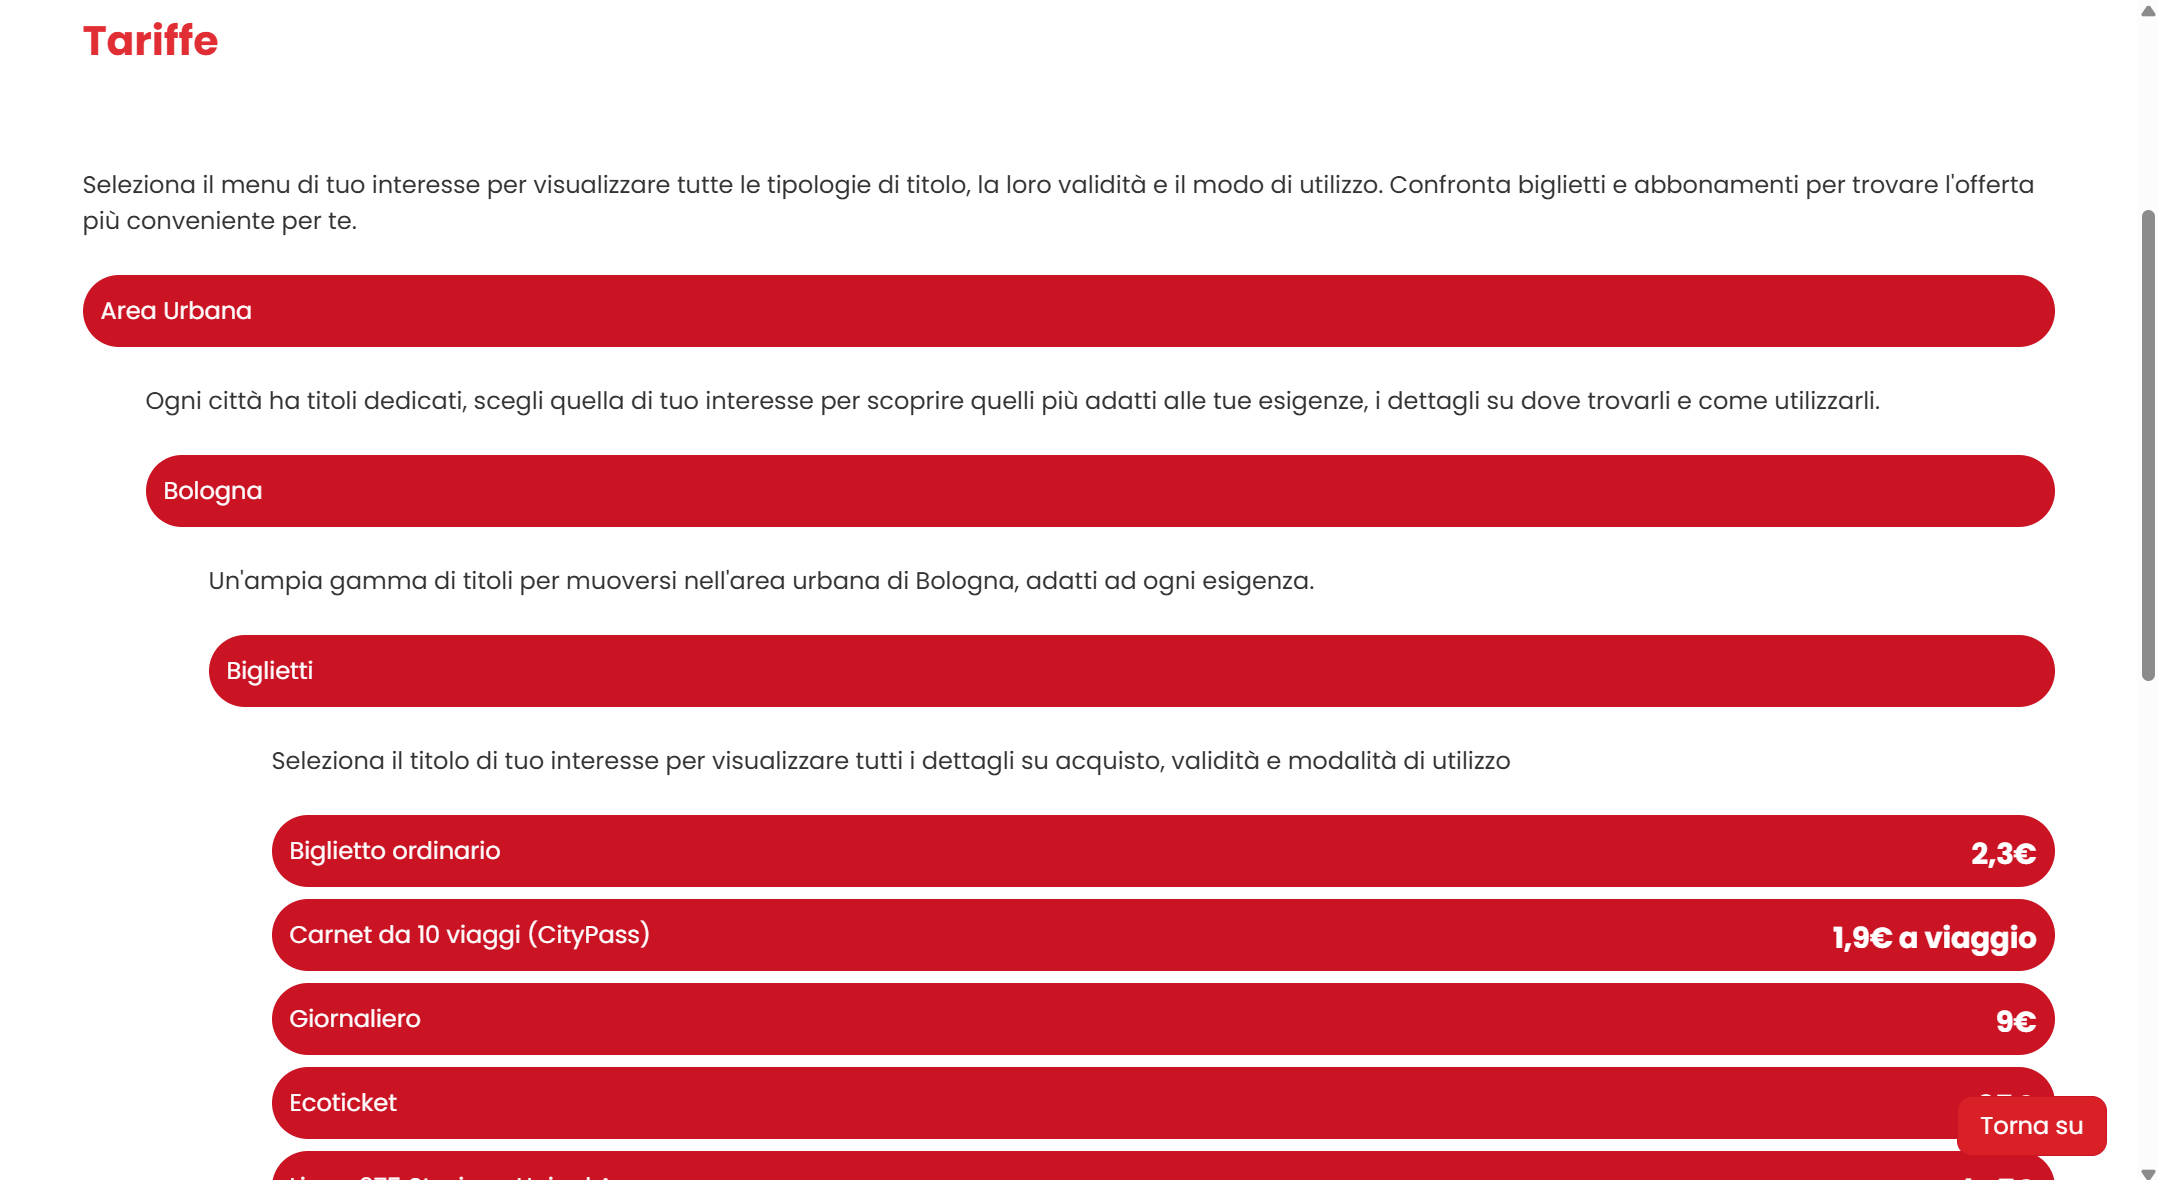
\includegraphics[width=0.332\textwidth]{Tper sito originale/Tariffe.png}\\[2pt]
{\small\textit{Biglietti \hspace{3.3cm} Abbonamenti \hspace{3.3cm} Tariffe}}\\[2pt]
{\footnotesize 3 pagine sovrapposte: contenuti duplicati, canali sepolti, terminologia aziendale}

\vspace{0.5cm}

\textbf{After --- Redesign tper 2.0}\\[4pt]
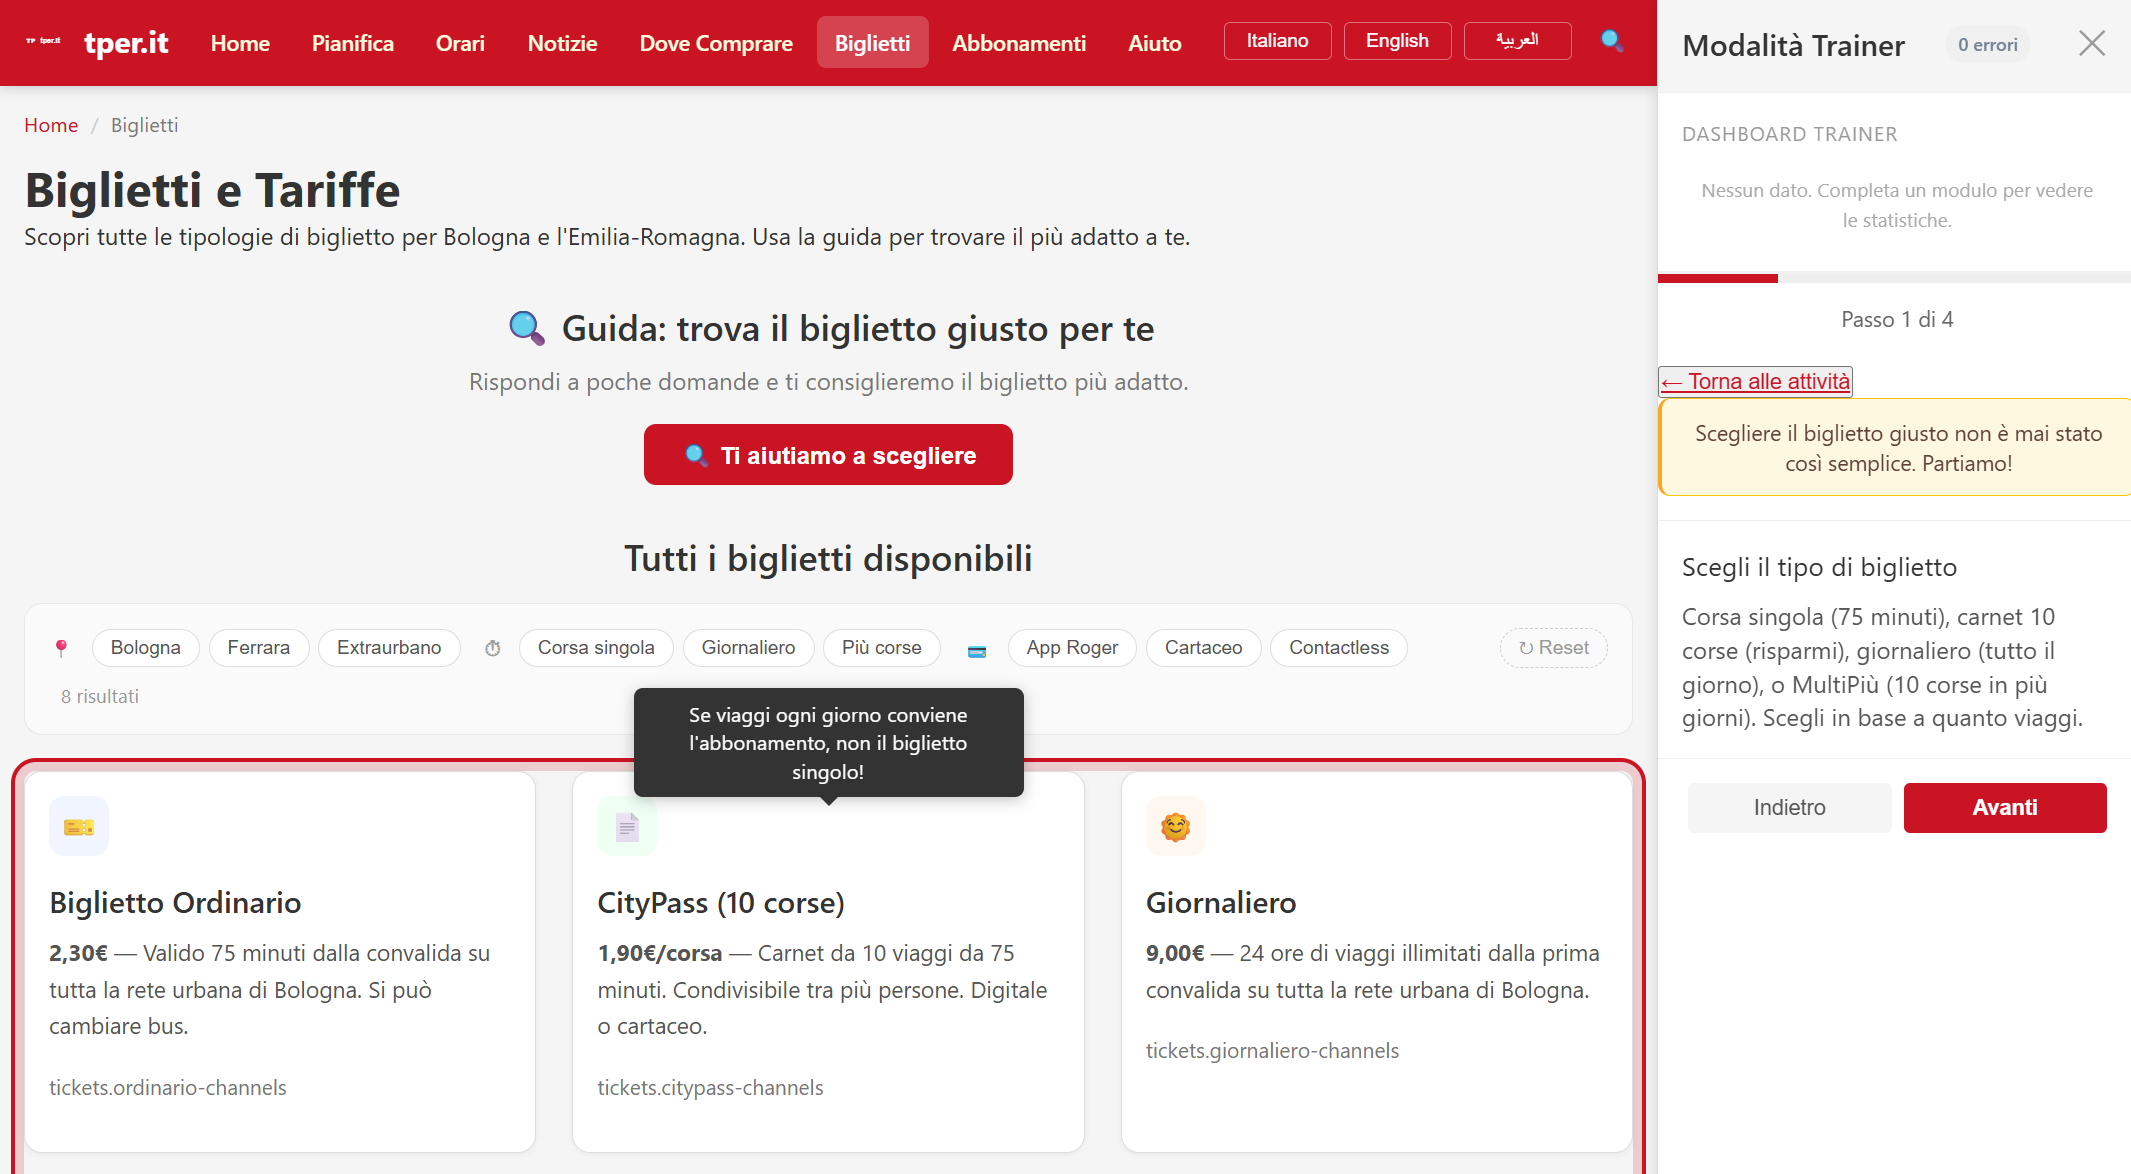
\includegraphics[width=0.332\textwidth]{Redesign Tper 2.0/Biglietti.png}\hfill
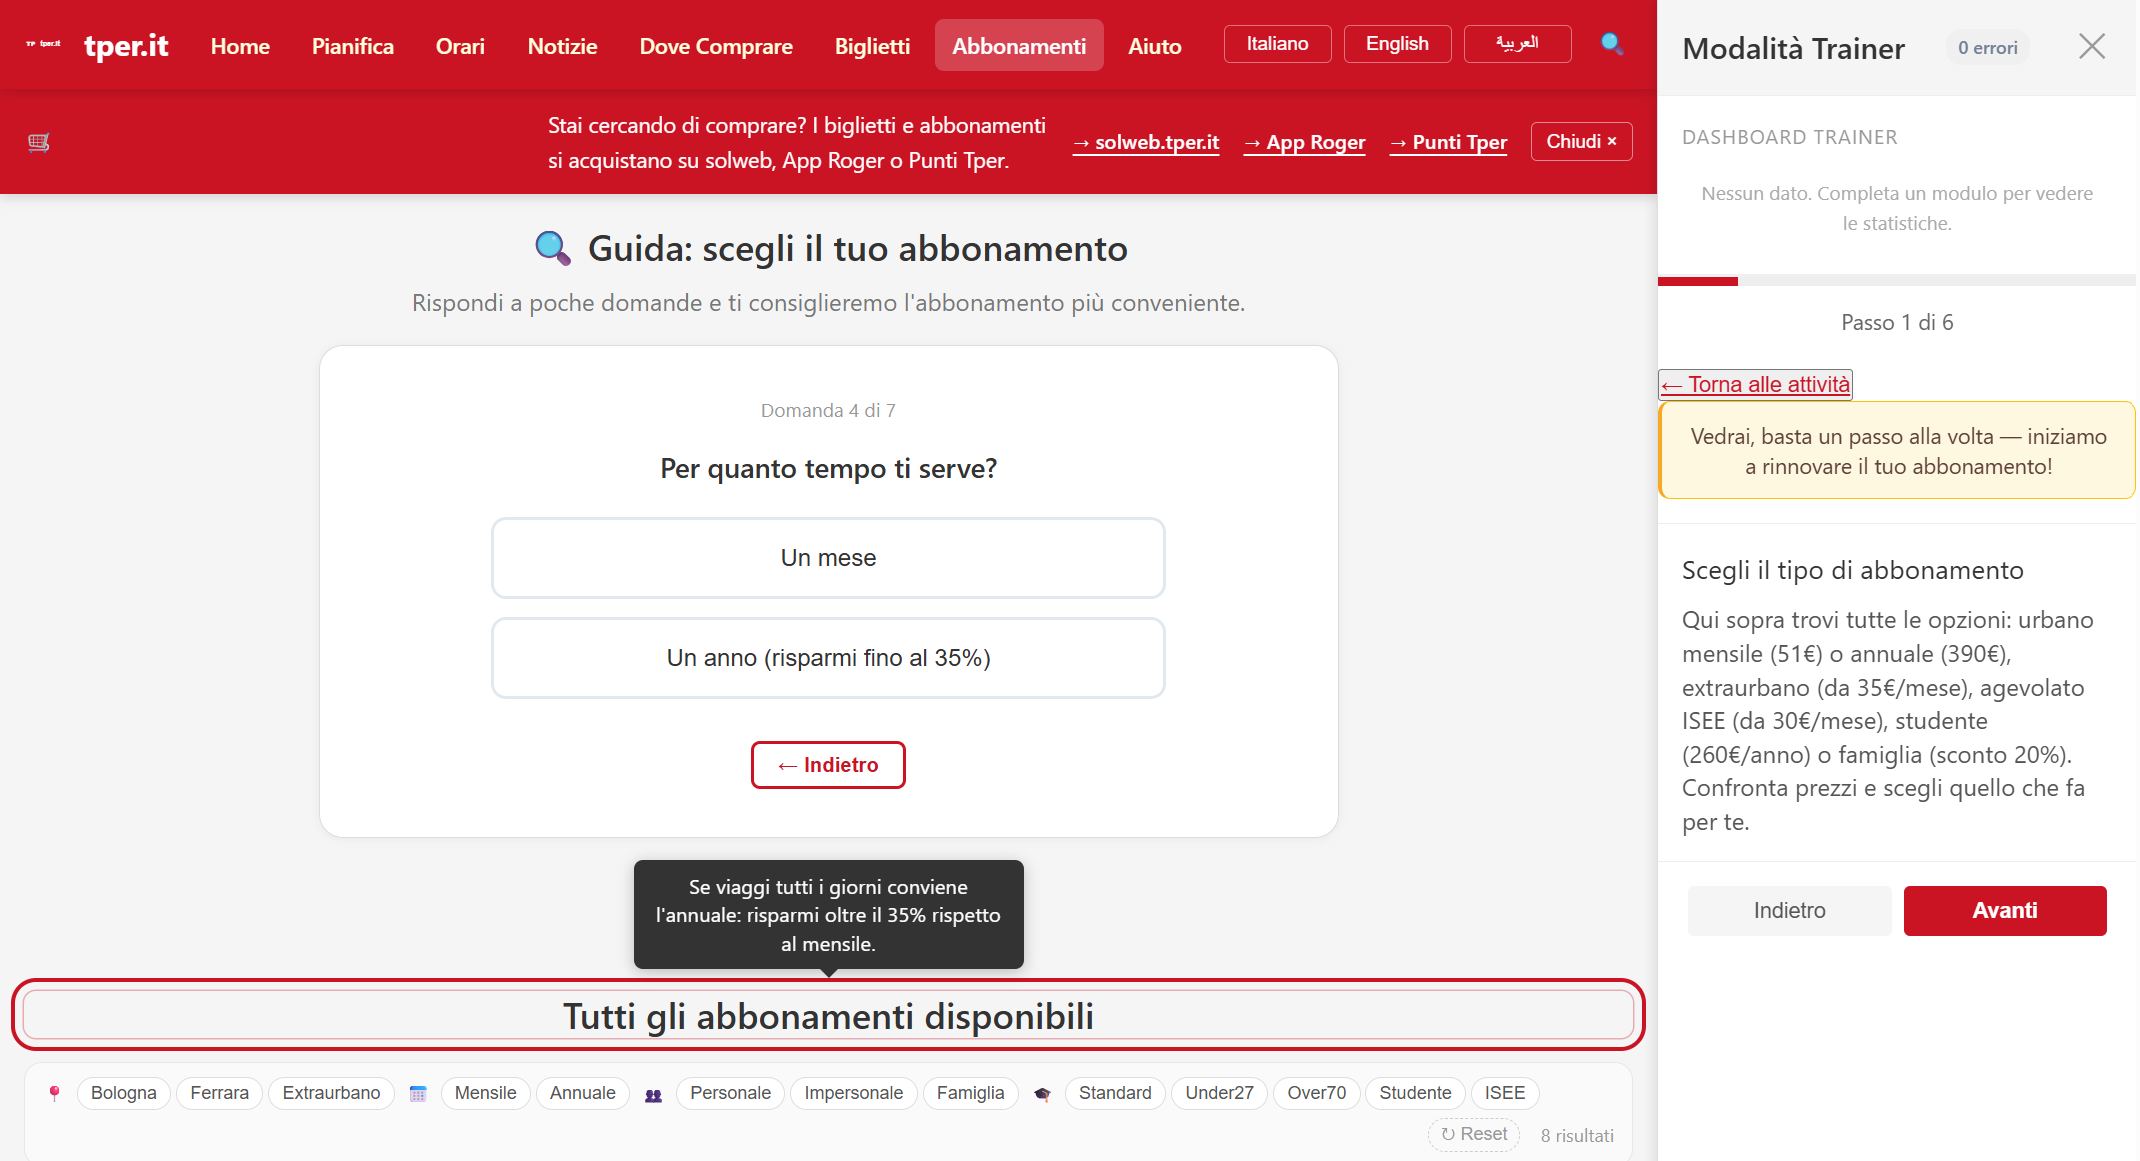
\includegraphics[width=0.332\textwidth]{Redesign Tper 2.0/Abbonamenti.png}\hfill
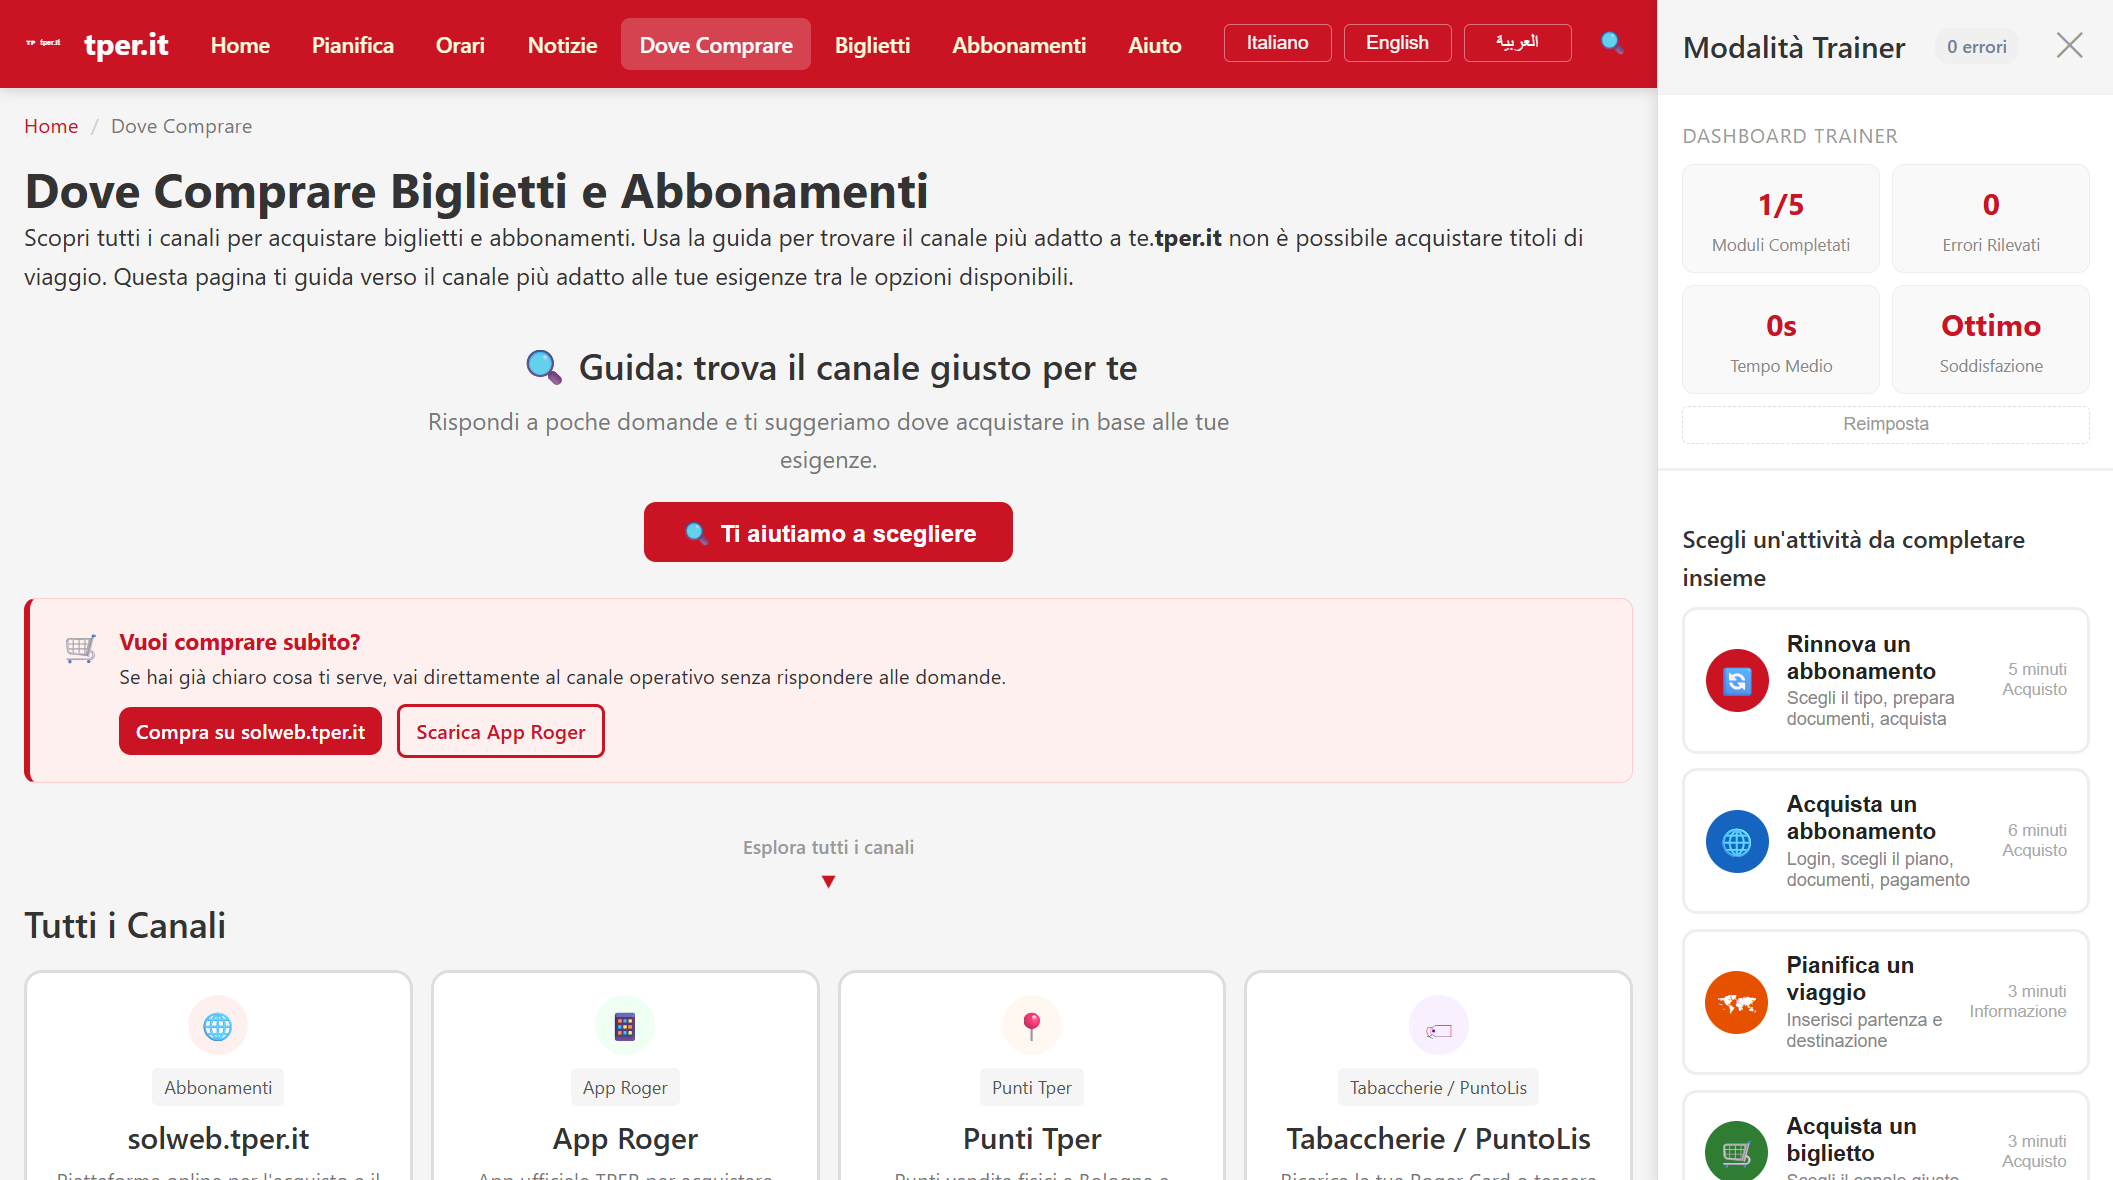
\includegraphics[width=0.332\textwidth]{Redesign Tper 2.0/Dove Comprare.png}\\[2pt]
{\small\textit{Biglietti \hspace{3.3cm} Abbonamenti \hspace{2.8cm} Dove Comprare}}\\[2pt]
{\footnotesize 3 pagine specializzate: ogni pagina ha un compito unico, tariffe integrate nei prodotti}

\caption{Confronto 3v3 --- Ristrutturazione dell'Architettura Informativa}
\label{fig:comparison-ia-3v3}
\end{figure}

\begin{table}[H]
\centering
\small
\renewcommand{\arraystretch}{1.4}
\begin{tabular}{|p{0.5cm}|p{7cm}|p{7cm}|}
\hline
& \textbf{Before (Originale)} & \textbf{After (Redesign 2.0)} \\ \hline
\cellcolor{primaryColor!15} &
\textit{3 pagine sovrapposte} &
\textit{3 pagine specializzate} \\ \hline

\raisebox{0.5cm}{\rotatebox{90}{\textbf{Struttura}}} &
3 pagine con contenuti duplicati e confini sfumati. Biglietti e Abbonamenti contengono entrambi riferimenti a tariffe e canali. La pagina Tariffe è ridondante. Navigazione a 3+ livelli per raggiungere la guida canali (D2). &
3 pagine con responsabilità chiare e distinte. Ogni pagina ha un unico compito. Nessuna duplicazione. Accesso diretto a ogni sezione dalla navigazione principale (max 1 click). Le tariffe sono mostrate nel contesto del prodotto (R2). \\ \hline

\raisebox{0.5cm}{\rotatebox{90}{\textbf{Biglietti}}} &
Elenca tipologie di biglietti, ma include anche informazioni sui canali di vendita e rimandi alle tariffe. L'utente non capisce se questa è la pagina giusta per decidere cosa comprare o dove comprarlo (D2, D3). &
Pagina focalizzata esclusivamente sui biglietti. Wizard a 5 domande (zona, frequenza, durata, app, compagnia). Pillole filtro per zona/validità/canale con contatore e reset. Banner informativo: ``tper.it è un sito informativo''. \\ \hline

\raisebox{0.5cm}{\rotatebox{90}{\textbf{Abbonamenti}}} &
Elenca piani di abbonamento con terminologia aziendale (MiMuovo, SaltaSu, Prontobus). Include canali e tariffe. Nessuna guida alla scelta: l'utente deve leggere tutte le opzioni e dedurre quale fa per lui (UR-05). &
Pagina focalizzata esclusivamente sugli abbonamenti. Wizard a 7 domande (azione, impersonale?, zona, durata, intestatario, agevolazione, canale). Filtro a 4 gruppi. Accordion ``Come Acquistare o Rinnovare''. Callout per verificare diritto a sconto (R9). \\ \hline

\raisebox{0.5cm}{\rotatebox{90}{\textbf{Canali / Tariffe}}} &
\textbf{Canali}: ``Rete di vendita'' sepolta sotto Biglietti e Abbonamenti, raggiungibile in 3 click. \textbf{Tariffe}: pagina separata con prezzi, scollegata dal contesto d'uso --- l'utente deve ricordare il prezzo mentre naviga altrove per decidere (D3). &
\textbf{Dove Comprare}: sezione autonoma e prominente nella navigazione principale. Wizard a 3 domande $\rightarrow$ canale consigliato con icona, descrizione e link diretto. Tabella comparativa 5 canali $\times$ 7 operazioni. \textbf{Tariffe}: integrate in Biglietti e Abbonamenti --- visibili nel momento della decisione (R2, R4). \\ \hline

\raisebox{0.5cm}{\rotatebox{90}{\textbf{Impatto}}} &
6/20 task completati (30\%). SUS medio 37.5/100. Maria B. (79 anni): 0/5 task, 652\,s medi, 13 errori per task. &
Dati Phase D: Laura P. 4/5 task (80\%), SUS 72.5 (+35 punti). T4 (agevolazioni): da 195\,s e 7 errori a 57\,s e 0 errori. La separazione delle responsabilità ha eliminato la confusione tra ``cosa comprare'' e ``dove comprare''. \\ \hline
\end{tabular}
\caption{Ristrutturazione IA: Biglietti, Abbonamenti e Canali}
\label{tab:comparison-ia-3v3}
\end{table}

\vspace{0.3cm}

% ============================================================
% CONFRONTO 4: FLUSSO ACQUISTO solweb
% ============================================================
\section{Flusso Acquisto \texttt{solweb.tper.it}}
\label{sec:comparison-acquisto}

\textbf{D4+D5 $\rightarrow$ R7+R10} --- No recupero errori $\rightarrow$ Messaggi guidati + guest path. Chris 498s, 8 errori, 10 backtrack su T3.

\begin{figure}[H]
\centering
\begin{minipage}[t]{0.498\textwidth}
\centering
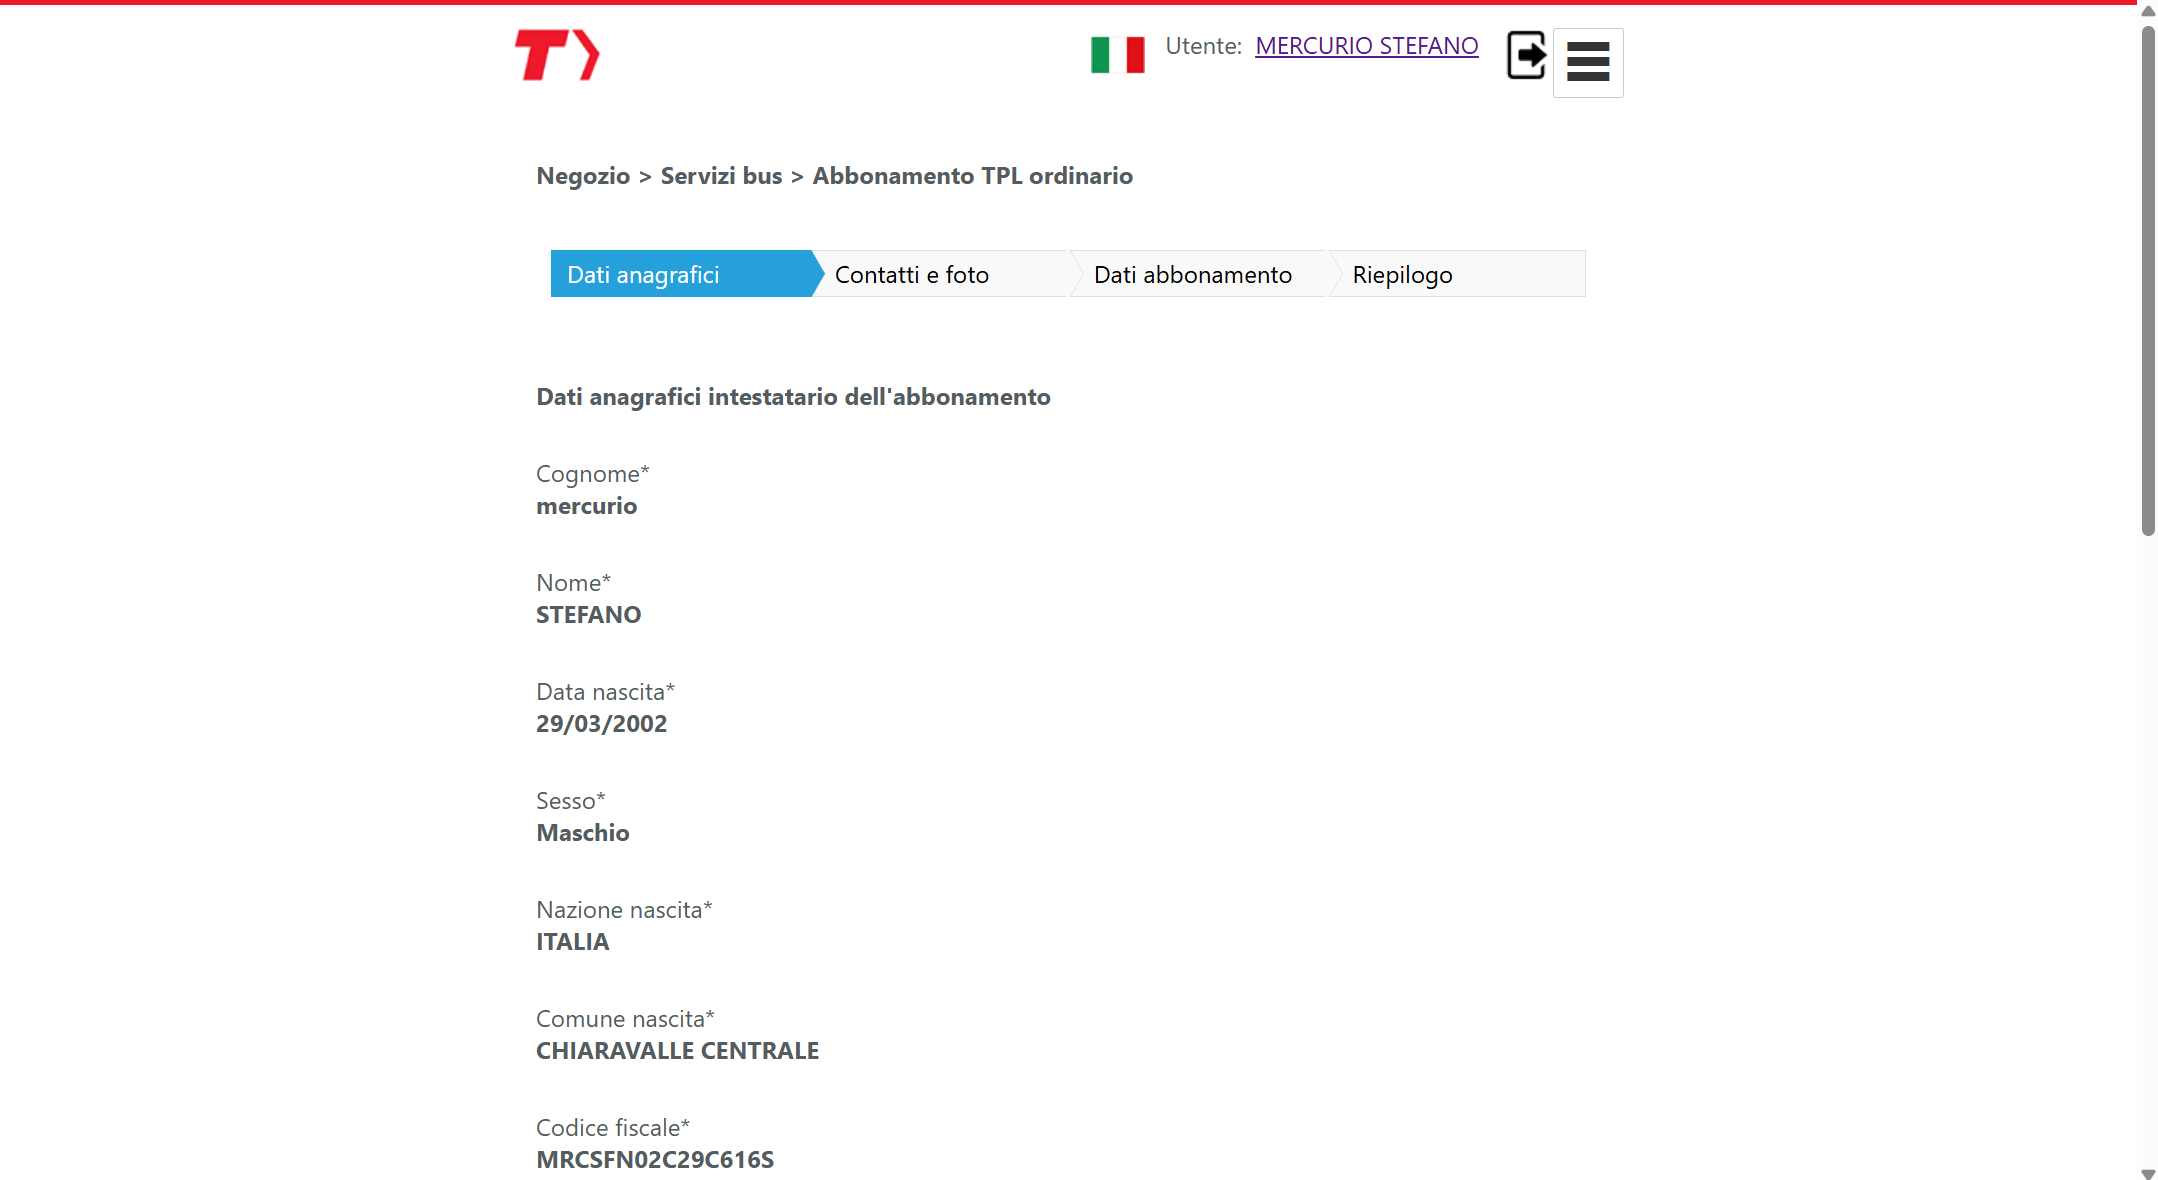
\includegraphics[width=\textwidth]{Tper sito originale/FlussoAcquistoS.png}
\par\small\textit{Before: flusso acquisto originale --- registrazione obbligatoria, nessuna guida}
\end{minipage}
\hfill
\begin{minipage}[t]{0.498\textwidth}
\centering
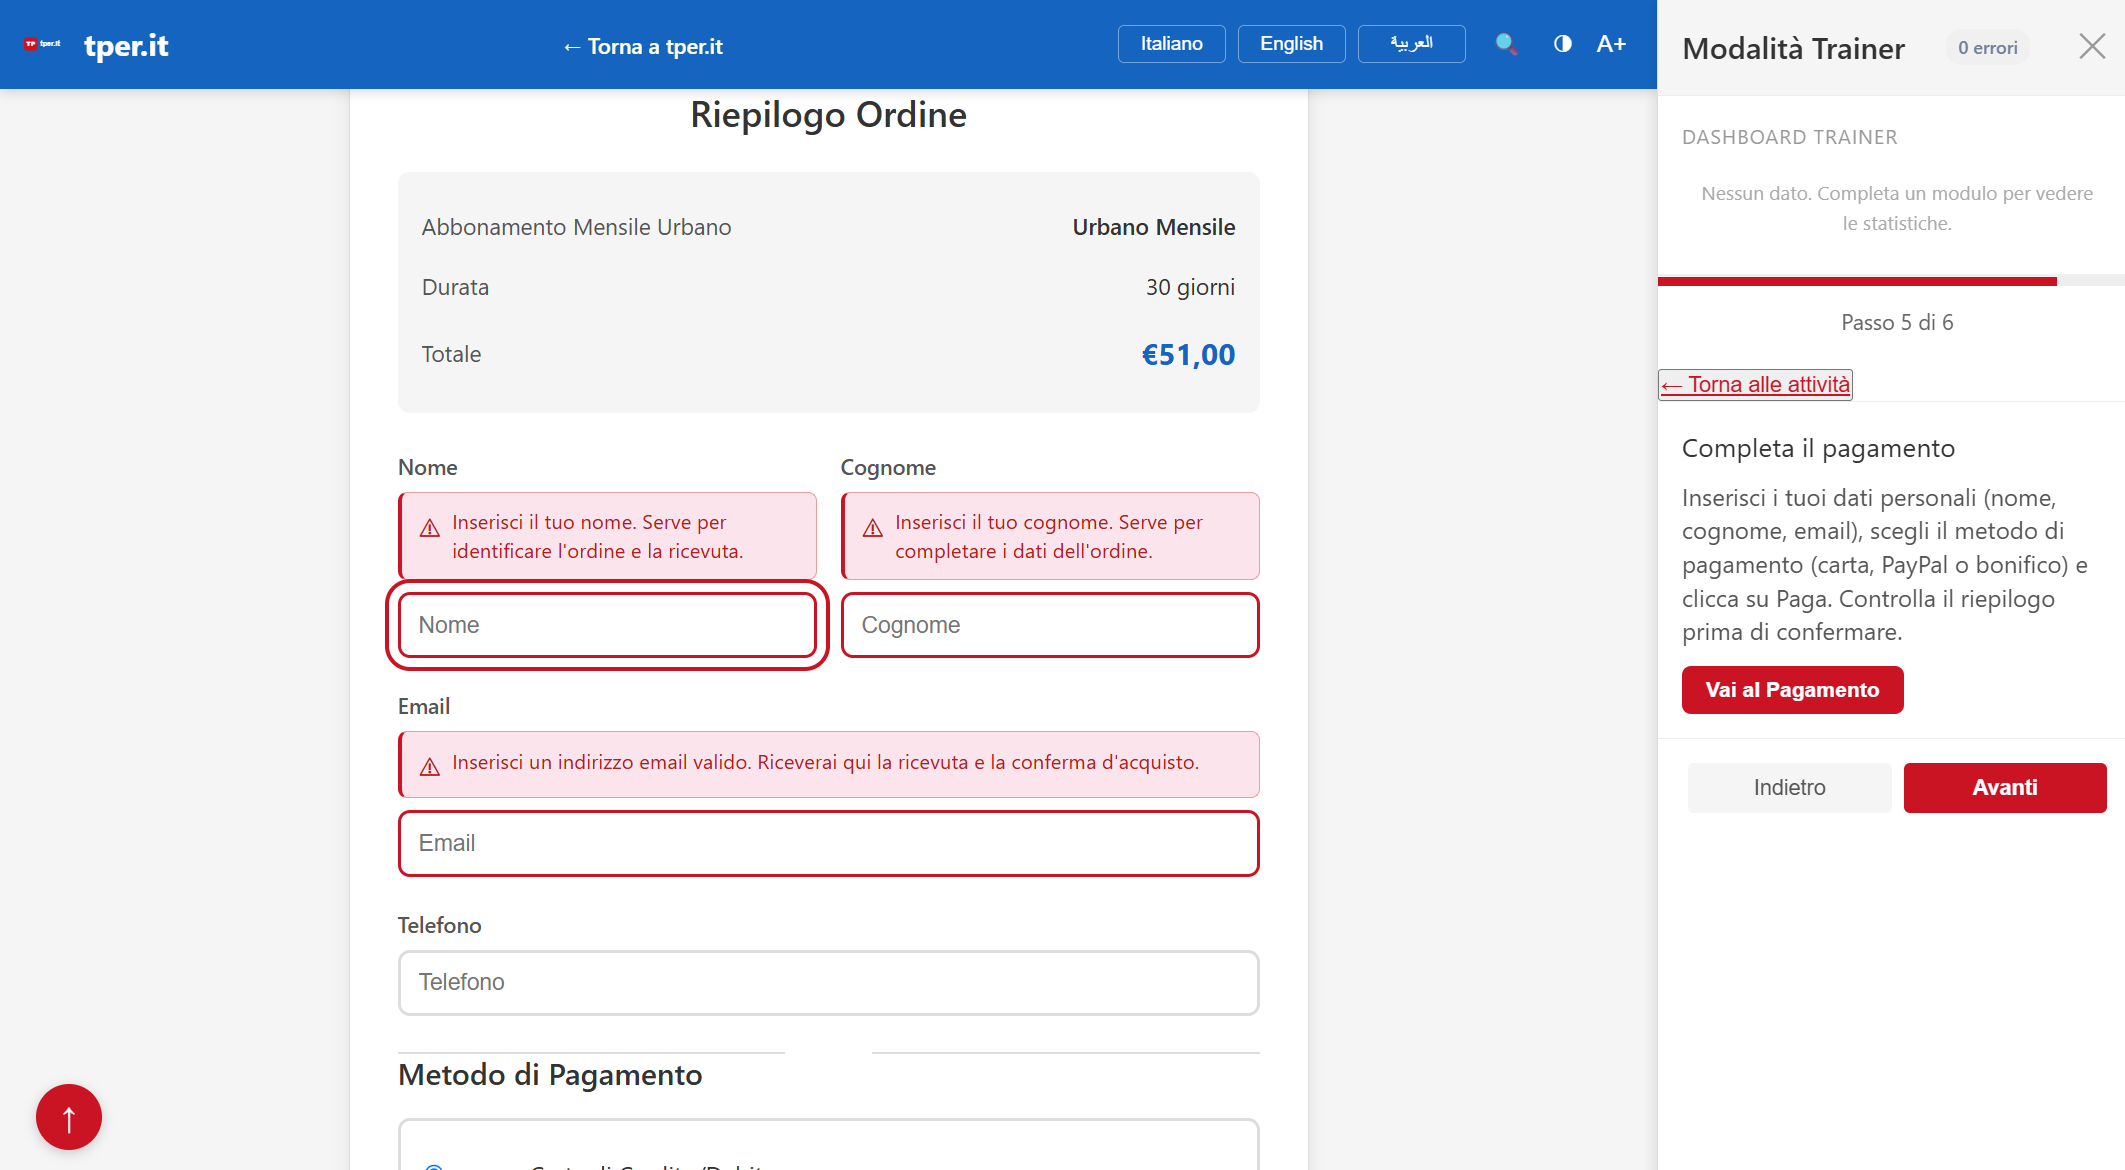
\includegraphics[width=\textwidth]{Redesign Tper 2.0/RiepilogoS.png}
\par\small\textit{After: flusso acquisto 2.0 --- barra progresso, form guidato, riepilogo}
\end{minipage}
\caption{Flusso Acquisto \texttt{solweb.tper.it}}
\label{fig:comparison-acquisto}
\end{figure}

\begin{table}[H]
\centering
\small
\renewcommand{\arraystretch}{1.4}
\begin{tabular}{|p{0.5cm}|p{7cm}|p{7cm}|}
\hline
& \textbf{Before} & \textbf{After} \\ \hline
\cellcolor{primaryColor!15} &
\textit{Flusso acquisto solweb originale} &
\textit{Flusso acquisto solweb 2.0} \\ \hline

\raisebox{0.5cm}{\rotatebox{90}{\textbf{Progresso}}} &
Nessun indicatore di progresso. L'utente non sa a che punto è del processo né quanti passi mancano. Abbandono frequente per disorientamento (Issue D2). &
\textbf{Barra di progresso a 4 passi}: Accedi $\rightarrow$ Scegli il Piano $\rightarrow$ Documenti $\rightarrow$ Pagamento. Ogni passo mostra: numero del passo, descrizione testuale, indicatore grafico di completamento (verde = completato, rosso = attivo). Visibile su tutte le pagine del flusso (R3). \\ \hline

\raisebox{0.5cm}{\rotatebox{90}{\textbf{Documenti}}} &
Nessuna checklist preventiva. L'utente scopre quali documenti servono solo dopo aver iniziato il flusso, spesso causando abbandono a metà. Utenti anziani costretti a tornare allo sportello perché privi dei documenti (R11). &
\textbf{Checklist interattiva} con barra di progresso (0/4 $\rightarrow$ 4/4). 4 card documento con riproduzione visiva del documento reale (dov'è il numero, dov'è la scadenza). Checkbox ``Ho questo documento''. Caricamento guidato. Badge ``Documenti necessari'' visibile prima di iniziare (R11). \\ \hline

\raisebox{0.5cm}{\rotatebox{90}{\textbf{Pagamento}}} &
Form di pagamento senza riepilogo ordine. Nessuna icona di sicurezza. Messaggi di errore generici: ``Errore --- riprovare''. L'utente non sa cosa ha sbagliato né come correggere (Issue D4). &
\textbf{Riepilogo ordine} sempre visibile: piano, durata, totale. 3 metodi di pagamento con radio button (Carta, PayPal, Bonifico). Checkbox termini. Messaggi di errore esponenziali: cosa è successo + perché + come risolvere + alternativa (R10). \\ \hline

\raisebox{0.5cm}{\rotatebox{90}{\textbf{Flessibilità}}} &
Unico percorso possibile: registrazione $\rightarrow$ login $\rightarrow$ acquisto. Nessuna variante per ricarica, rinnovo impersonale o sanzioni (Issue D5). &
\textbf{Multi-flusso}: pagamento.html gestisce 4 flussi diversi (acquisto, rinnovo, ricarica, sanzioni) con breadcrumb e form adattivi. Il percorso guest per rinnovo impersonale e ricarica salta completamente la registrazione (R7). \\ \hline
\end{tabular}
\caption{Flusso Acquisto solweb}
\label{tab:comparison-acquisto}
\end{table}

\vspace{0.3cm}

% ============================================================
% CONFRONTO 5: RIEPILOGO POST-ACQUISTO
% ============================================================
\section{Riepilogo Post-Acquisto \texttt{solweb.tper.it}}
\label{sec:comparison-riepilogo}

\textbf{UR-02 $\rightarrow$ R6} --- PDF scambiato per biglietto valido $\rightarrow$ 3 passi guidati post-acquisto. Rischio multa a bordo.

\begin{figure}[H]
\centering
\begin{minipage}[t]{0.498\textwidth}
\centering
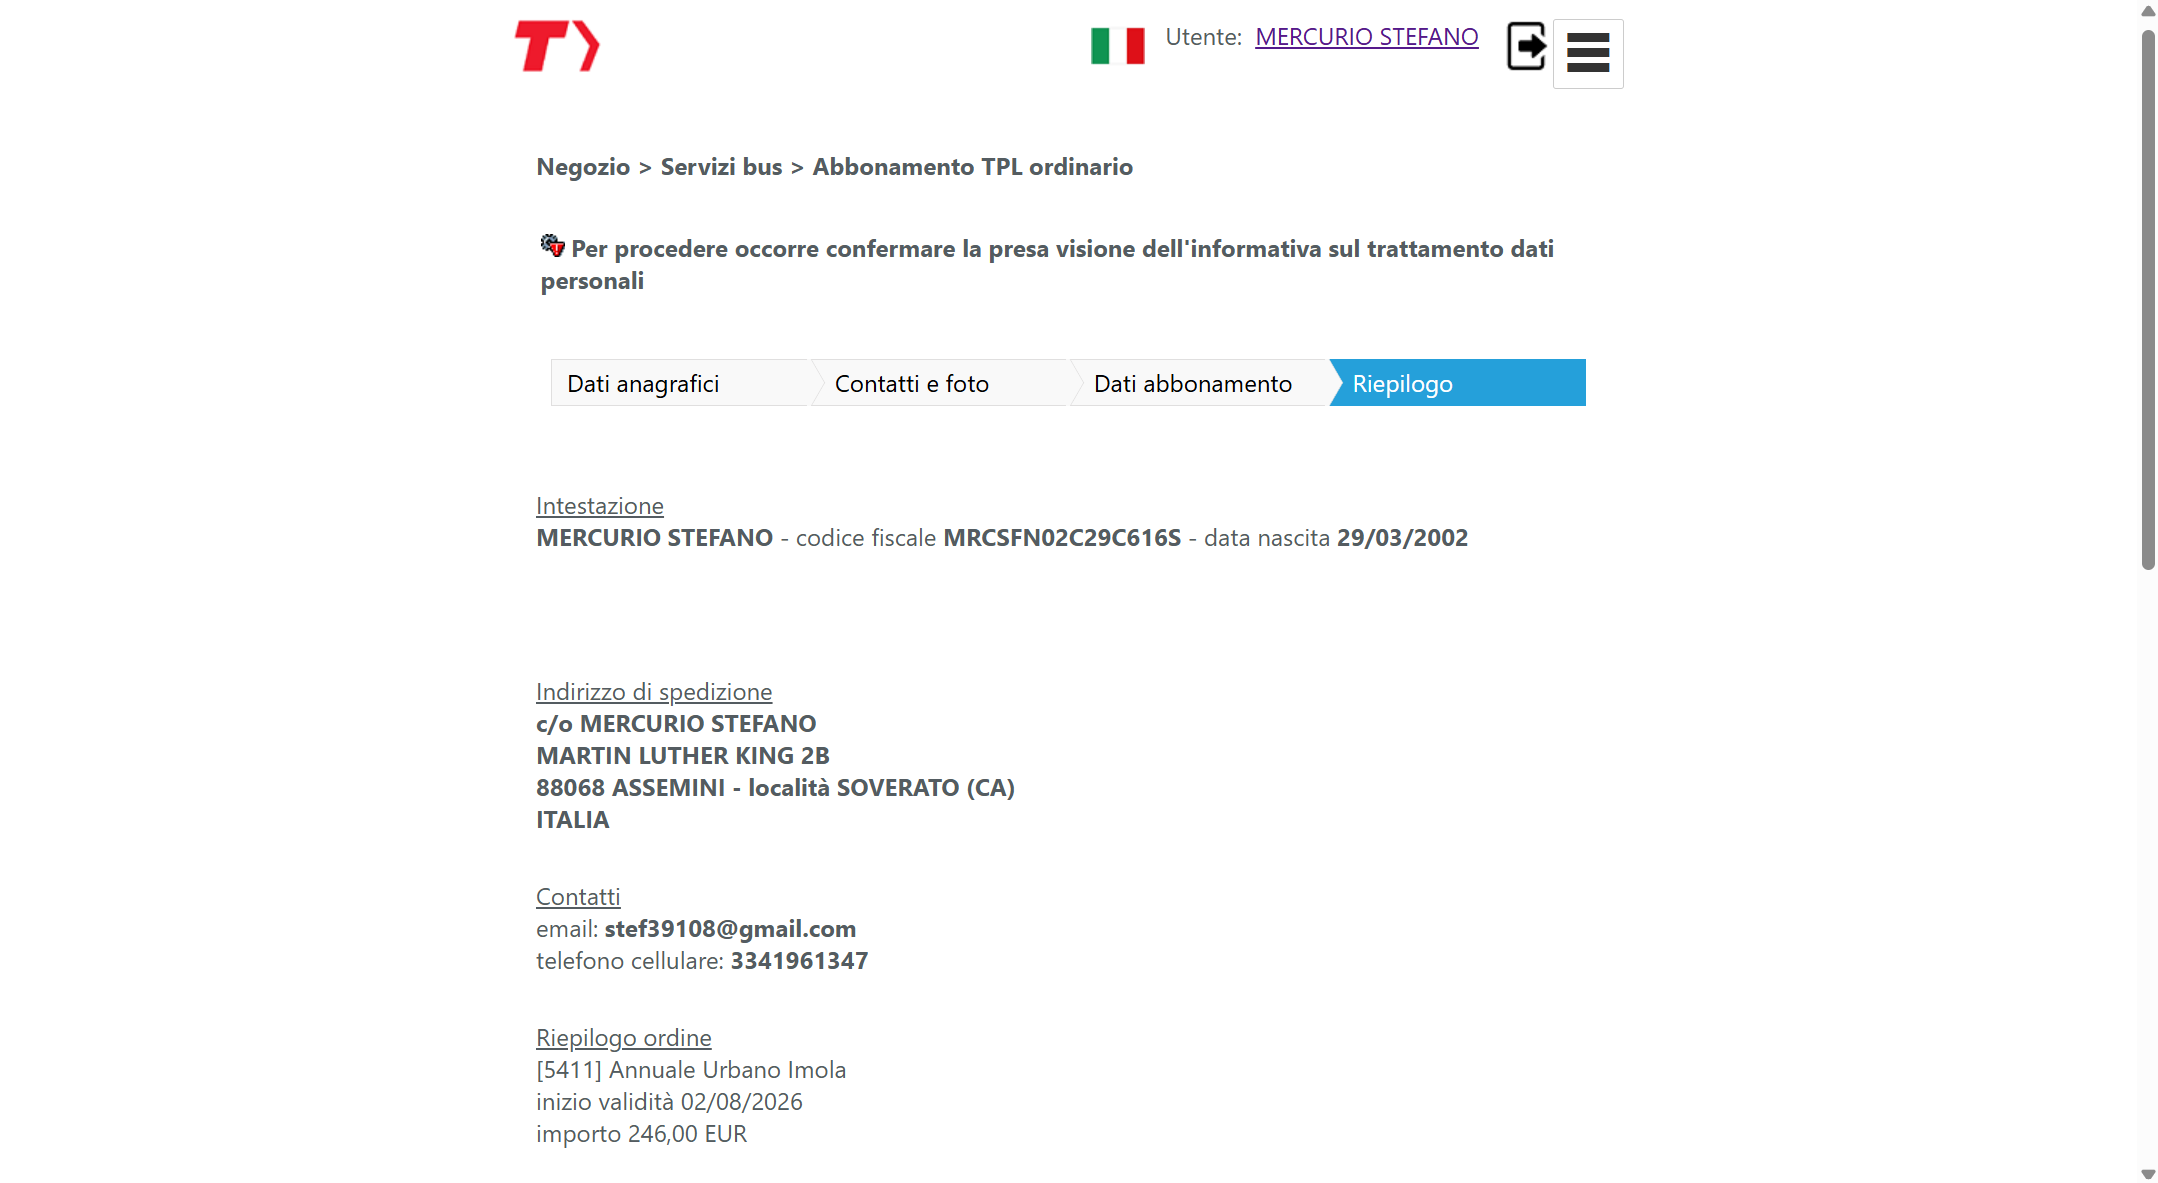
\includegraphics[width=\textwidth]{Tper sito originale/RiepilogoS.png}
\par\small\textit{Before: riepilogo originale --- solo conferma, nessuna guida post-acquisto}
\end{minipage}
\hfill
\begin{minipage}[t]{0.498\textwidth}
\centering
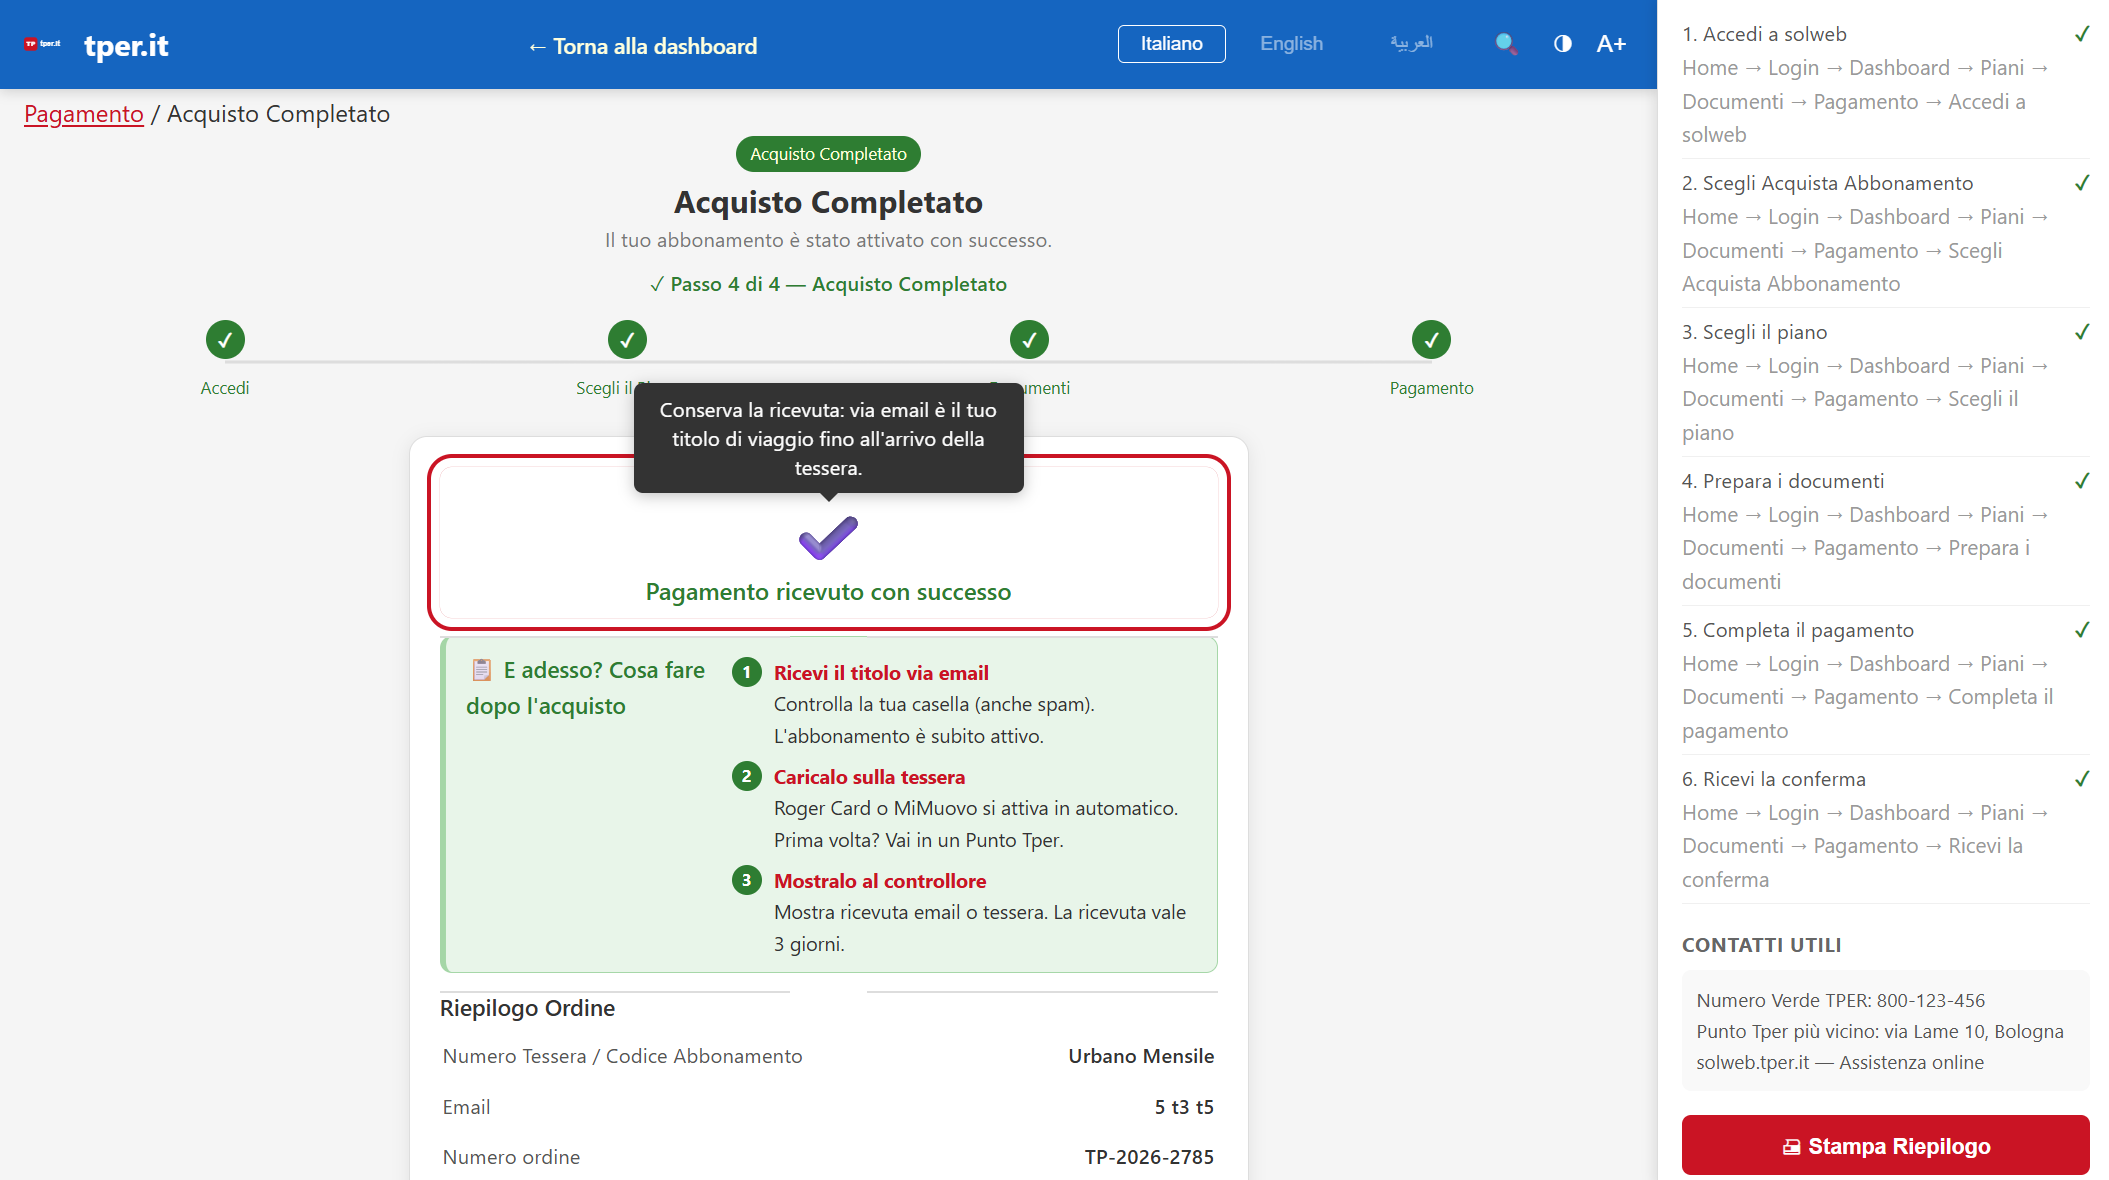
\includegraphics[width=\textwidth]{Redesign Tper 2.0/AcquistoS.png}
\par\small\textit{After: conferma 2.0 --- 3 passi guidati + ricevuta stampabile}
\end{minipage}
\caption{Riepilogo Post-Acquisto}
\label{fig:comparison-riepilogo}
\end{figure}

\begin{table}[H]
\centering
\small
\renewcommand{\arraystretch}{1.4}
\begin{tabular}{|p{0.5cm}|p{7cm}|p{7cm}|}
\hline
& \textbf{Before} & \textbf{After} \\ \hline
\cellcolor{primaryColor!15} &
\textit{Riepilogo originale post-acquisto} &
\textit{Conferma post-acquisto in solweb 2.0} \\ \hline

\raisebox{0.5cm}{\rotatebox{90}{\textbf{Conferma}}} &
Messaggio scarno di conferma. Nessuna spiegazione di cosa accade dopo. Il PDF generato viene scambiato per un titolo di viaggio valido --- ma non lo è (UR-02). &
\textbf{H1}: ``Grazie per il tuo acquisto!''. Barra di progresso completa (4/4 con spunta verde). Riepilogo ordine dettagliato: piano, email, numero ordine, metodo di pagamento, totale. Pulsante ``Scarica Ricevuta (PDF)'' (R6). \\ \hline

\raisebox{0.5cm}{\rotatebox{90}{\textbf{Istruzioni}}} &
\textbf{Assenti.} Nessuna guida su come utilizzare il biglietto/abbonamento acquistato. L'utente non sa se deve stampare qualcosa, mostrare il telefono, o validare una tessera (UR-02). &
\textbf{3 passi guidati post-acquisto}: (1) Riceverai una email di conferma con i dettagli dell'ordine, (2) La tua tessera si attiverà automaticamente entro 24 ore, (3) Mostra la tessera al controllore a bordo. Ogni passo è numerato e illustrato con icone (R6, UR-02). \\ \hline

\raisebox{0.5cm}{\rotatebox{90}{\textbf{Supporto}}} &
Nessun link di supporto post-acquisto. L'utente in difficoltà deve cercare autonomamente il servizio clienti. &
Link all'aiuto sempre visibile. Riferimento al numero ordine per assistenza. Possibilità di tornare alla dashboard o alla home. \\ \hline

\raisebox{0.5cm}{\rotatebox{90}{\textbf{Multicanale}}} &
Nessuna connessione con altri canali. Il percorso termina senza indicazioni su come usare il servizio acquistato su Roger, al Punto Tper o a bordo. &
Riferimenti cross-canale: se hai acquistato un abbonamento, ti spieghiamo come usarlo anche sull'App Roger. Se hai pagato una sanzione, ti indichiamo come verificare lo stato (UR-02, R6). \\ \hline
\end{tabular}
\caption{Riepilogo Post-Acquisto}
\label{tab:comparison-riepilogo}
\end{table}

\vspace{0.3cm}

% ============================================================
% CONFRONTO 6: TRAINER MODE E SUPPORTO
% ============================================================
\section{Trainer Mode e Supporto}
\label{sec:comparison-trainer}

\textbf{R5 $\rightarrow$ R4+R5+R6} --- Nessun trainer $\rightarrow$ Sidebar 22 pagine, 5 moduli, script operatore. Maria 0/5 task, SUS 27.5.

\begin{figure}[H]
\centering
\begin{minipage}{0.498\textwidth}
\centering
\rule{\textwidth}{0.1pt}
\vspace{2cm}
\rule{\textwidth}{0.1pt}
\par\small\textit{Before: nessun trainer mode --- solo help desk telefonico}
\end{minipage}
\hfill
\begin{minipage}[t]{0.498\textwidth}
\centering
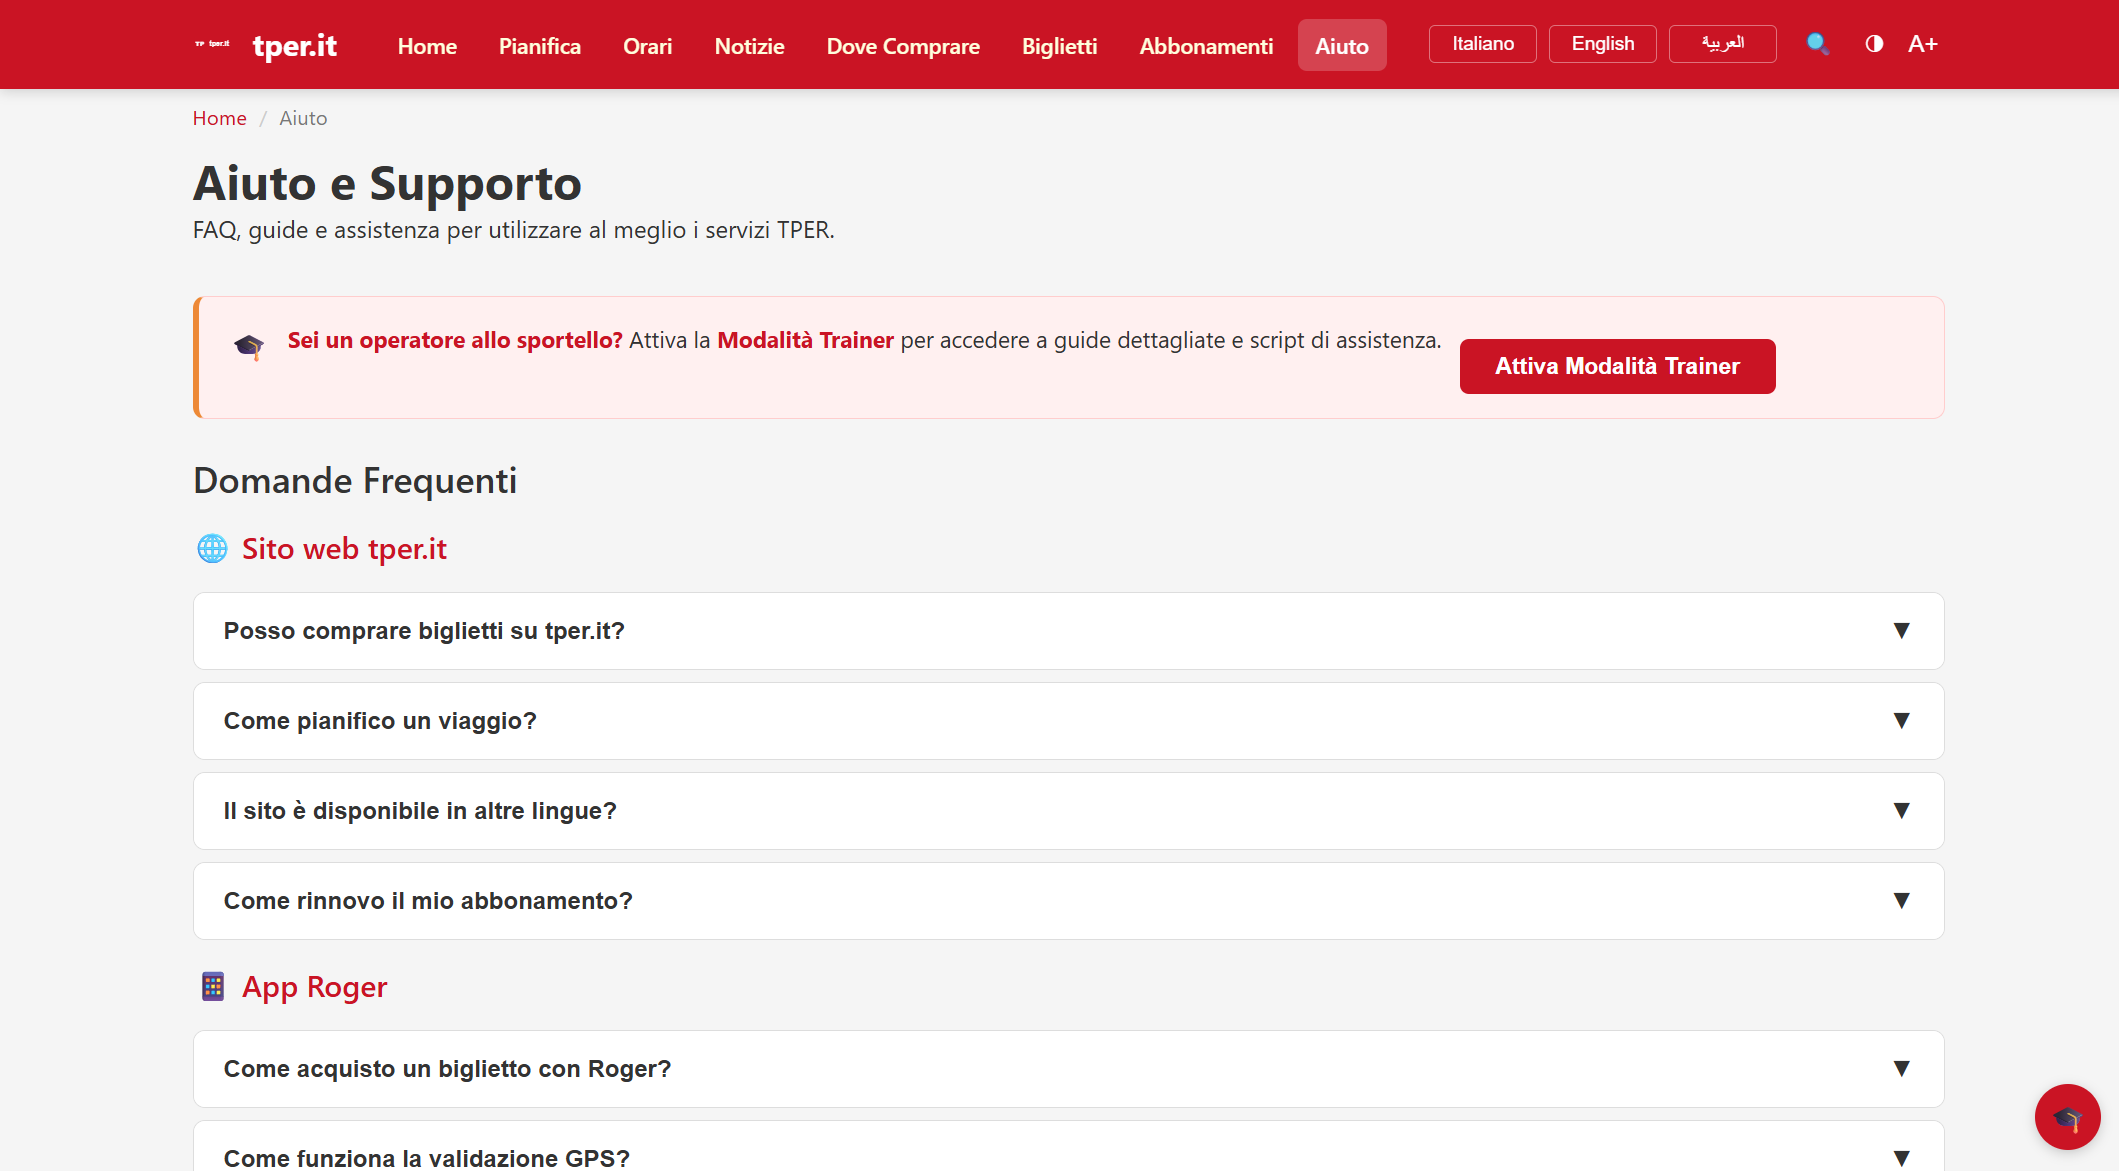
\includegraphics[width=\textwidth]{Redesign Tper 2.0/Aiuto.png}
\par\small\textit{After: sezione Aiuto con trainer mode, FAQ, guide passo-passo}
\end{minipage}
\caption{Trainer Mode e Supporto}
\label{fig:comparison-trainer}
\end{figure}

\begin{table}[H]
\centering
\small
\renewcommand{\arraystretch}{1.4}
\begin{tabular}{|p{0.5cm}|p{7cm}|p{7cm}|}
\hline
& \textbf{Before} & \textbf{After} \\ \hline
\cellcolor{primaryColor!15} &
\textit{Supporto attuale su \texttt{tper.it}} &
\textit{Trainer-mode e supporto in tper 2.0} \\ \hline

\raisebox{0.5cm}{\rotatebox{90}{\textbf{Trainer}}} &
\textbf{Inesistente.} Nessuna modalità assistita per operatori allo sportello. Nessun meccanismo di guida passo-passo per accompagnare utenti a bassa competenza digitale nell'orientamento tra i canali. L'unico canale di supporto è il servizio clienti (telefonico o email) (R4, R5). &
\textbf{Barra laterale integrata} su tutte le 22 pagine del sito. 5 moduli trainer: Rinnovo, Acquista, Viaggio, Biglietto, Ricarica. Ogni modulo carica automaticamente la pagina corretta con gli highlight sugli elementi rilevanti. Attivazione: su richiesta (pulsante $\mathcal{T}$) o automatica dopo 2 errori consecutivi dell'utente (R4, R5). \\ \hline

\raisebox{0.5cm}{\rotatebox{90}{\textbf{Script}}} &
Nessuno script operativo per il personale di sportello. &
Script a 5 passi per operatori: (1) Identifica il bisogno, (2) Consiglia il titolo di viaggio, (3) Indirizza al canale corretto, (4) Spiega la validazione, (5) Conferma e chiedi se serve altro (R4). \\ \hline

\raisebox{0.5cm}{\rotatebox{90}{\textbf{FAQ}}} &
Solo help desk come canale di supporto. Nessuna guida interattiva, nessun FAQ organizzato (R10). &
\textbf{Accordion FAQ raggruppato per canale}: \texttt{tper.it}, App Roger, Punti Tper e Rivendite, Sanzioni, Contactless a Bordo. Ogni sezione risponde alle domande più comuni per quel canale. Include link diretti (es. da FAQ solweb $\rightarrow$ pagina di acquisto) (R9, R10). \\ \hline

\raisebox{0.5cm}{\rotatebox{90}{\textbf{Guide}}} &
Assenti. &
3 card guida passo-passo nella sezione Aiuto: ``Come acquistare su solweb'', ``Come usare Roger App'', ``Come trovare un Punto Tper''. Ciascuna con CTA diretta al canale corrispondente. Wizard interattivi su Dove Comprare, Biglietti e Abbonamenti (R9). \\ \hline

\raisebox{0.5cm}{\rotatebox{90}{\textbf{Persistenza}}} &
Nessuna memoria di sessione. Se l'utente chiude il browser o scade il timeout, perde tutto e deve ricominciare da capo. &
\textbf{Auto-salvataggio} dello stato della sessione trainer in localStorage. L'utente può riprendere dal punto esatto in cui si era interrotto. Riepilogo stampabile con screenshot annotati e percorso di navigazione (R5, R6). \\ \hline
\end{tabular}
\caption{Trainer Mode e Supporto}
\label{tab:comparison-trainer}
\end{table}

\vspace{0.3cm}

% ============================================================
% CONFRONTO 7: ACCESSIBILITÀ E MULTILINGUA
% ============================================================
\section{Accessibilità e Multilingua}
\label{sec:comparison-a11y}

\textbf{R3+D3 $\rightarrow$ R8+R12} --- Solo IT, 10pt, target <44px $\rightarrow$ IT/EN/AR, 14pt, WCAG AA. Chris 3/5 falliti per lingua.

\begin{table}[H]
\centering
\small
\renewcommand{\arraystretch}{1.4}
\begin{tabular}{|p{0.5cm}|p{7cm}|p{7cm}|}
\hline
& \textbf{Before} & \textbf{After} \\ \hline
\cellcolor{primaryColor!15} &
\textit{Stato attuale del sito \texttt{tper.it} live} &
\textit{Accessibilità e lingue in tper 2.0} \\ \hline

\raisebox{0.5cm}{\rotatebox{90}{\textbf{Lingua}}} &
\textbf{Solo italiano.} Nessun selettore di lingua, nessun contenuto in inglese o arabo. Utenti stranieri completamente esclusi dai servizi informativi online. Chris H. (inglese): 3/5 task falliti nonostante alta competenza digitale (R12). &
\textbf{IT + EN + AR.} Commutatore lingua a tre pulsanti sempre visibile nell'header di ogni pagina. Traduzione completa delle label, dei contenuti informativi, delle FAQ e dei wizard. 1.600+ chiavi i18n nei file JavaScript. Supporto RTL per l'arabo (R12). \\ \hline

\raisebox{0.5cm}{\rotatebox{90}{\textbf{Carattere}}} &
Testo piccolo (10--11pt). Difficoltà di lettura per utenti over 65, particolarmente critico per i nomi dei canali e le tariffe. Maria B. non distingueva pulsanti da testo statico (R8). &
\textbf{Minimo 14pt} su tutti i testi. Pulsante \textbf{A+} nell'header per ingrandire ulteriormente il carattere con un click. Toggle persistente tra le pagine (R8). \\ \hline

\raisebox{0.5cm}{\rotatebox{90}{\textbf{Contrasto}}} &
Contrasto non dichiarato, verosimilmente inferiore allo standard WCAG AA per alcune combinazioni colore. &
\textbf{Rapporto minimo 4.5:1} (WCAG AA). Pulsante \textbf{$\blacksquare$} per attivare/disattivare la modalità contrasto elevato su tutte le pagine. Toggle persistente. Palette completamente rivista in modalità alto contrasto (R8). \\ \hline

\raisebox{0.5cm}{\rotatebox{90}{\textbf{ARIA}}} &
Skip link ``Salta al contenuto principale'' presente. Ruoli ARIA assenti o parziali sulla maggior parte degli elementi interattivi. &
\textbf{ARIA completo}: \texttt{role="banner"}, \texttt{role="navigation"}, \texttt{role="main"}, \texttt{role="complementary"} (trainer bar), \texttt{role="contentinfo"} (footer), \texttt{role="dialog"} (modali e search overlay), \texttt{role="search"} (route planner), \texttt{aria-label} su tutti gli elementi interattivi, \texttt{aria-current="page"} sulla pagina attiva, \texttt{aria-expanded} su hamburger e accordion, \texttt{aria-modal="true"} su overlay e modali (R8). \\ \hline

\raisebox{0.5cm}{\rotatebox{90}{\textbf{Target}}} &
Touch target inferiori a 44$\times$44px in molte aree, rendendo difficile l'uso su smartphone per utenti con ridotta destrezza. &
\textbf{Tutti i target interattivi $\ge$ 44$\times$44px} (WCAG 2.1). Pulsanti, link, checkbox e radio button dimensionati per interazione tattile senza errori (R8). \\ \hline
\end{tabular}
\caption{Accessibilità e Multilingua}
\label{tab:comparison-a11y}
\end{table}

\vspace{0.3cm}

% ============================================================
% CONFRONTO 8: TONO E TERMINOLOGIA
% ============================================================
\section{Tono e Terminologia}
\label{sec:comparison-tone}

\textbf{D3 $\rightarrow$ R9} --- Terminologia aziendale $\rightarrow$ Linguaggio utente + glosse. ``MiMuovo'', ``Rete di vendita'' incomprensibili a tutti i soggetti.

\begin{table}[H]
\centering
\small
\renewcommand{\arraystretch}{1.4}
\begin{tabular}{|p{0.5cm}|p{7cm}|p{7cm}|}
\hline
& \textbf{Before} & \textbf{After} \\ \hline
\cellcolor{primaryColor!15} &
\textit{Linguaggio attuale su \texttt{tper.it}} &
\textit{Tono e terminologia in tper 2.0} \\ \hline

\raisebox{0.5cm}{\rotatebox{90}{\textbf{Tono}}} &
Burocratico e istituzionale. Frasi impersonali, lessico da pubblica amministrazione. Messaggi di errore freddi e generici. L'utente si sente un ``praticante'' piuttosto che un cliente (Issue D3). &
Incoraggiante e inclusivo. Linguaggio in prima persona plurale: ``Ti aiutiamo a scegliere'', ``Nessun problema, possiamo riprovare insieme''. Messaggi di errore con tono umano e via d'uscita: ``Non hai trovato quello che cercavi? Prova con una di queste alternative'' (R9). \\ \hline

\raisebox{0.5cm}{\rotatebox{90}{\textbf{Termini}}} &
Terminologia esclusivamente aziendale: \textit{Rete di vendita}, \textit{Emettitrici automatiche}, \textit{MiMuovo}, \textit{SaltaSu}, \textit{Prontobus}, \textit{Discobus}. \texttt{solweb} e \textit{Roger} mai spiegati né introdotti. L'utente deve conoscere il gergo TPER prima di usare il sito (Issue D3). &
\textbf{Terminologia utente-centrica con glosse}: ``Dove Comprare'' (non ``Rete di vendita''), ``Abbonamenti online (solweb)'', ``Biglietti digitali (Roger)'', ``Tabaccherie e PuntoLis''. Ogni termine tecnico è accompagnato da una spiegazione inline o da un tooltip al primo utilizzo. Il nome aziendale resta tra parentesi per riferimento (R2, R9). \\ \hline

\raisebox{0.5cm}{\rotatebox{90}{\textbf{Messaggi}}} &
Messaggi di sistema impersonali e privi di guida. ``Errore --- riprovare'' senza spiegazione di causa o soluzione. L'utente abbandona il flusso (Issue D4). &
\textbf{Messaggi esponenziali} (R10): cosa è successo, perché è successo, come risolvere, cosa fare in alternativa. Box con sfondo a contrasto e icona di avviso, posizionato inline sopra il campo interessato. Micro-rinforzi dopo ogni passo: ``Perfetto, questo è fatto!'' (R9). \\ \hline

\raisebox{0.5cm}{\rotatebox{90}{\textbf{Onboarding}}} &
Nessun percorso di primo accesso. L'utente arriva sulla homepage e deve capire tutto da solo. Maria B.: \textit{``non so neanche da dove cominciare''}. &
\textbf{Tour ``Prima Volta''}: 4 schermate illustrate che spiegano i canali tramite metafore quotidiane. Attivabile dal pulsante Aiuto. Linguaggio rassicurante: ``Non preoccuparti, ti spiego dove andare'' (R9). \\ \hline
\end{tabular}
\caption{Tono e Terminologia}
\label{tab:comparison-tone}
\end{table}

\vspace{0.5cm}

% ============================================================
% RIEPILOGO
% ============================================================
\section{Riepilogo delle Differenze Chiave}
\label{sec:comparison-summary}

\begin{tcolorbox}[colback=backgroundColor,colframe=primaryColor,arc=2mm]
{\small
\renewcommand{\arraystretch}{1.3}
\begin{tabular}{|p{3.5cm}|p{5cm}|p{5cm}|}
\hline
\textbf{Dimensione} & \textbf{Before (\texttt{tper.it} live)} & \textbf{After (tper 2.0)} \\ \hline
Homepage \texttt{tper.it} & News aziendali e slider istituzionale (D1) & Hero pianificatore + griglia 6 card task-oriented (R1) \\ \hline
Homepage \texttt{solweb} & Solo login, nessun percorso guest (D5) & 4 azioni rapide senza registrazione + progress bar (R7) \\ \hline
Architettura Informativa & 3 pagine sovrapposte (Biglietti, Abbonamenti, Tariffe), canali sepolti al 3\textdegree{} livello (D2) & 3 pagine specializzate: Biglietti, Abbonamenti, Dove Comprare --- ogni pagina, un compito (R2) \\ \hline
Navigazione & Mega-menu 200+ voci, 5 livelli di profondità & Nav flat 8 voci + breadcrumb su tutte le pagine \\ \hline
``Dove Comprare'' & Inesistente --- \textit{Rete di vendita} sepolta & Sezione autonoma + wizard 3 domande + tabella comparativa 5$\times$7 \\ \hline
solweb / Roger & Mai menzionati in homepage & Card dedicate con CTA dirette e modale di transizione \\ \hline
Guida canali & Assente --- scelta affidata all'utente & Wizard interattivi su 3 pagine + tabella comparativa \\ \hline
Flusso acquisto & Senza progresso, senza checklist documenti & Barra 4 passi + checklist interattiva (R3, R11) \\ \hline
Post-acquisto & Nessuna istruzione, PDF scambiato per biglietto (UR-02) & 3 passi guidati + ricevuta stampabile (R6) \\ \hline
Trainer Mode & Inesistente (R5) & Barra laterale su 22 pagine + 5 moduli + persistenza + riepilogo (R4, R5, R6) \\ \hline
FAQ / Guide & Solo help desk & Accordion per canale + 3 guide passo-passo + script operatore \\ \hline
Lingua & Solo italiano & IT + EN + AR, 1.600+ chiavi i18n, supporto RTL (R12) \\ \hline
Carattere / Contrasto & 10--11pt, sotto WCAG AA & 14pt min, 4.5:1, toggle A+, toggle contrasto (R8) \\ \hline
ARIA / Touch target & Parziale, target $<$ 44px & Completo: ruoli, label, stati; tutti i target $\ge$ 44$\times$44px (R8) \\ \hline
Tono & Burocratico/istituzionale & Incoraggiante/inclusivo + micro-rinforzi (R9) \\ \hline
Terminologia & Aziendale (Rete di vendita, MiMuovo, Emettitrici) & Utente-centrica con glosse (Dove Comprare, Abbonamenti online) \\ \hline
Errori & Messaggi generici ``Errore --- riprovare'' & Messaggi esponenziali: causa + soluzione + alternativa (R10) \\ \hline
Messaggio informativo & Assente & Banner ``tper.it è un sito informativo'' su ogni pagina (R1) \\ \hline
Documenti & Nessuna checklist preventiva & Checklist interattiva con riproduzione visiva (R11) \\ \hline
Guest path & Inesistente --- login obbligatorio per tutto & Rinnovo impers., ricarica, sanzioni senza registrazione (R7) \\ \hline
\end{tabular}
}
\end{tcolorbox}

\vspace{0.5cm}

\begin{center}
{\color{secondaryColor}\small
Documento compilato sulla base dell'analisi diretta dei siti \texttt{tper.it} e \texttt{solweb.tper.it} live, \\
delle raccomandazioni R1--R13 della Phase B, e dei risultati dei test utente Phase A (4 soggetti, SUS 37.5/100) \\[4pt]
\textbf{Phase C --- Design Proposal: Before/After Comparison} \\[4pt]
Progetto: UX Design Project: Help People Help People --- TPER S.p.A.}
\end{center}
